\documentclass[a4paper,12pt]{article}


\usepackage{graphicx}
\usepackage{amsmath}   
\usepackage{caption}       
\usepackage{xepersian}
\usepackage{setspace}
\usepackage{perpage}
\MakePerPage{footnote}



\renewcommand{\contentsname}{فهرست مطالب\\}
\numberwithin{figure}{subsection}
\settextfont[Extension=.ttf]{IRNazanin}

\begin{document}

\begin{titlepage}

    \centering
   \vspace*{-3cm}
    
    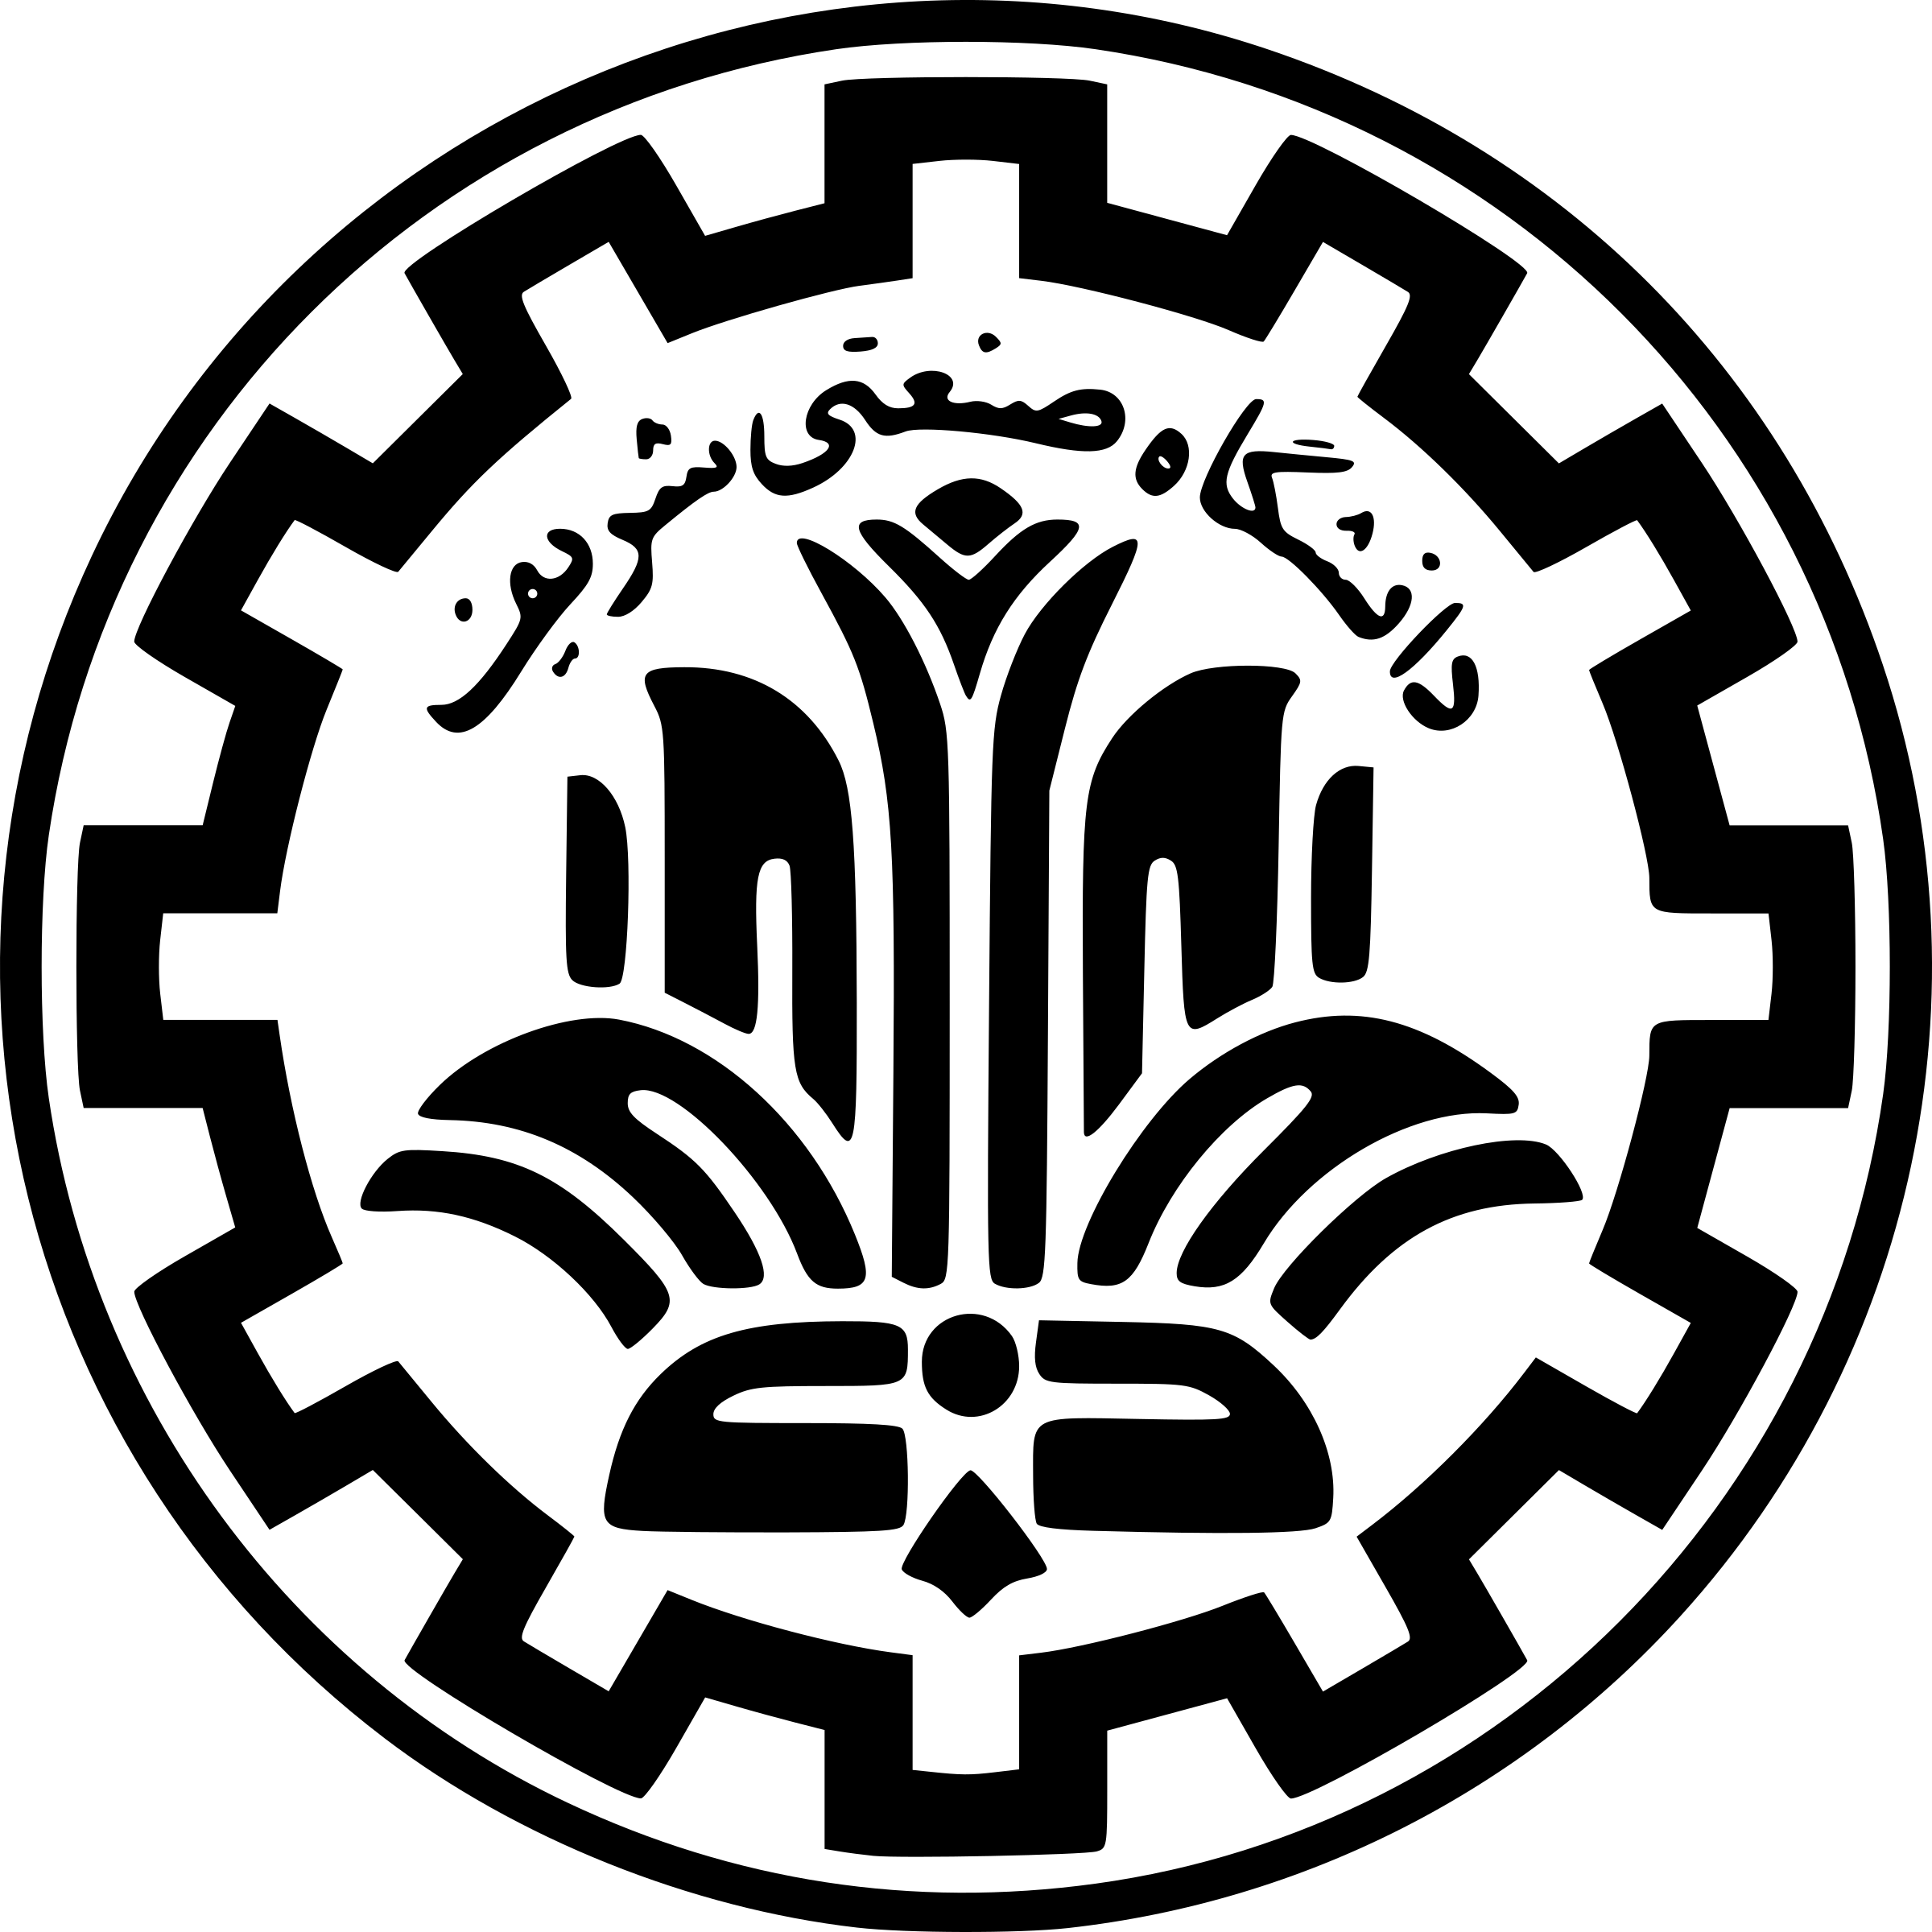
\includegraphics[width=4cm]{images/logo.png} 
    \\[1cm] % This adds 1cm of space below the logo
    
    
    {\Large \textbf{گزارش آزمایش}}\\[0.3cm]
    {\Large آزمایشگاه مدار منطقی}\\[1.5cm]
    
    {\LARGE \textbf{آزمایش اول}}\\[0.5cm]
    {\huge \textbf{آشنایی با محیط‌های شبیه‌سازی}}\\[2.5cm]
    
    % Group Members Table
    \begin{table}[h]
        \centering
        \large
        

        اعضای گروه:\\
        \vspace{0.5cm}
        \renewcommand{\arraystretch}{1.5} % Adds vertical padding to the rows
        \begin{tabular}{|c|c|}
            \hline
            \textbf{نام و نام خانوادگی} & \textbf{شماره دانشجویی} \\
            \hline
           روناک ابوطالبی & 404105394 \\
            \hline
            حسین مرادی & 404106366 \\
            \hline
        \end{tabular}
    \end{table}
    
    \vspace{2.5cm}
    
    {\large \textbf{تاریخ تحویل: 1405/05/14}}\\[1cm]
    
    {\large \textbf{تابستان 1405}}\\[1cm]
    
    \vfill
    
\end{titlepage}

\newpage
\begin{spacing}{1.5} 
    \tableofcontents 
\end{spacing}


\newpage
\section{مقدمه}
\leavevmode\par


\begin{spacing}{1.3}
هدف در این آزمایش این است که با سه نرم‌افزار طراحی و شبیه‌سازی مدارهای منظقی آشنا شویم. نرم‌افزار‌های مذکور عبارت‌اند از:\\
\end{spacing}

\vspace{-0.6cm}
\begin{latin}
\begin{itemize}
	\item Fritzing
	\item Logisim
	\item Proteus
\end{itemize}
\end{latin}

\begin{spacing}{1.3}
در قسمت اول، از نرم‌افزار \lr{Fritzing} استفاده می‌کنیم تا با بردبورد\LTRfootnote{Breadboard}، اتصالات و نحوه عمکرد آن آشنا شویم. در قسمت دوم، از نرم‌افزار \lr{Logisim} برای رسم کردن و تست یک مدار ترکیبی استفاده می‌کنیم و در نهایت‌، در بخش آخر، مدار دیگری را با استفاده از نرم‌افزار \lr{Proteus} می‌سازیم.
\end{spacing}

\newpage

\section{رسم مدار با \lr{Fritzing}}
\leavevmode\par

\vspace{0.3cm}



\begin{spacing}{1.3}

	\subsection{آشنایی با بردبورد}
	\leavevmode\par
	\vspace{0.2cm}
	
ابتدا می‌خواهیم با اتصالات بردبورد و نحوه کار با آن آشنا شویم.

\end{spacing}


\begin{figure}[h]    
    \centering
    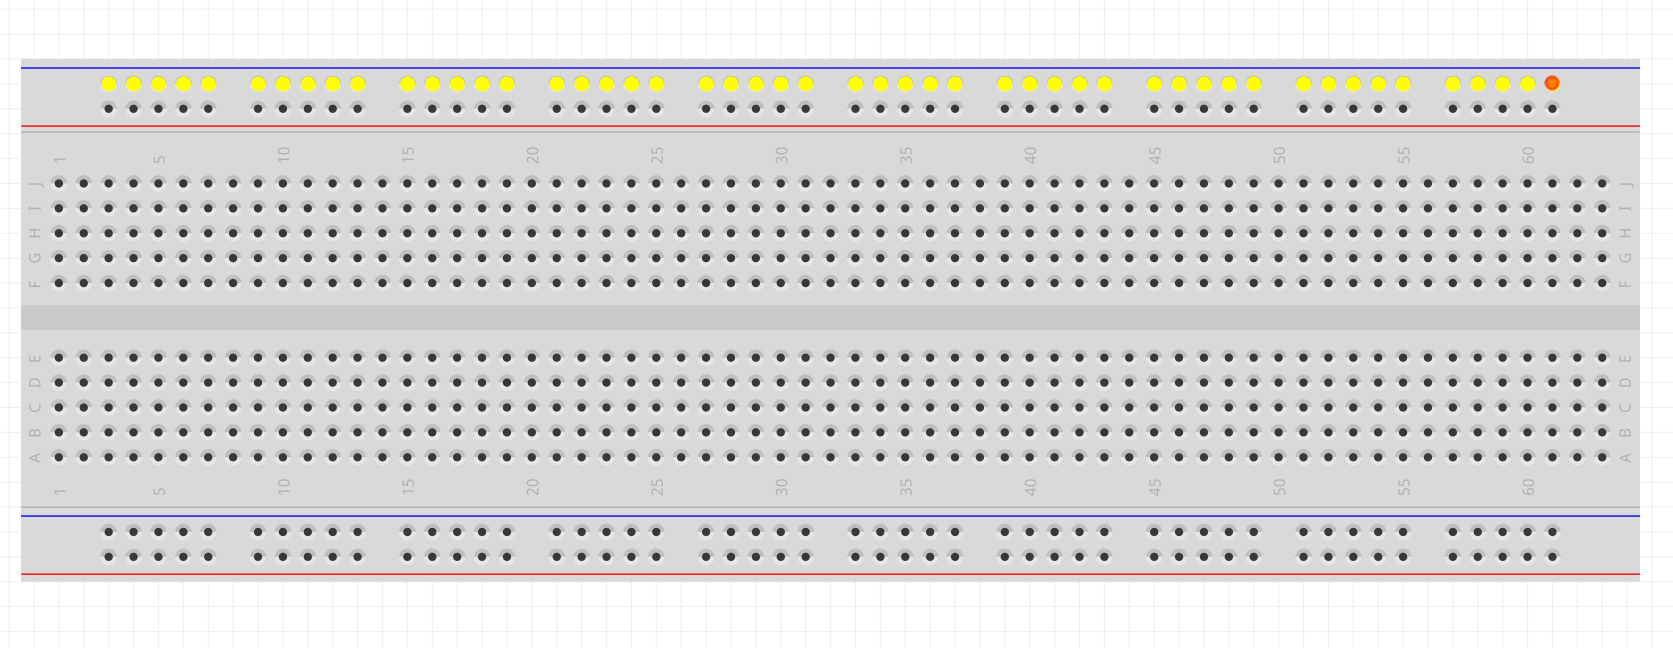
\includegraphics[width=0.9\textwidth]{images/Fritzing/breadboard1.png}
    \caption{جفت‌ردیف‌های افقی بالا و پایین}
    \label{fig:breadboard1}
\end{figure}

\begin{figure}[h]    
    \centering
    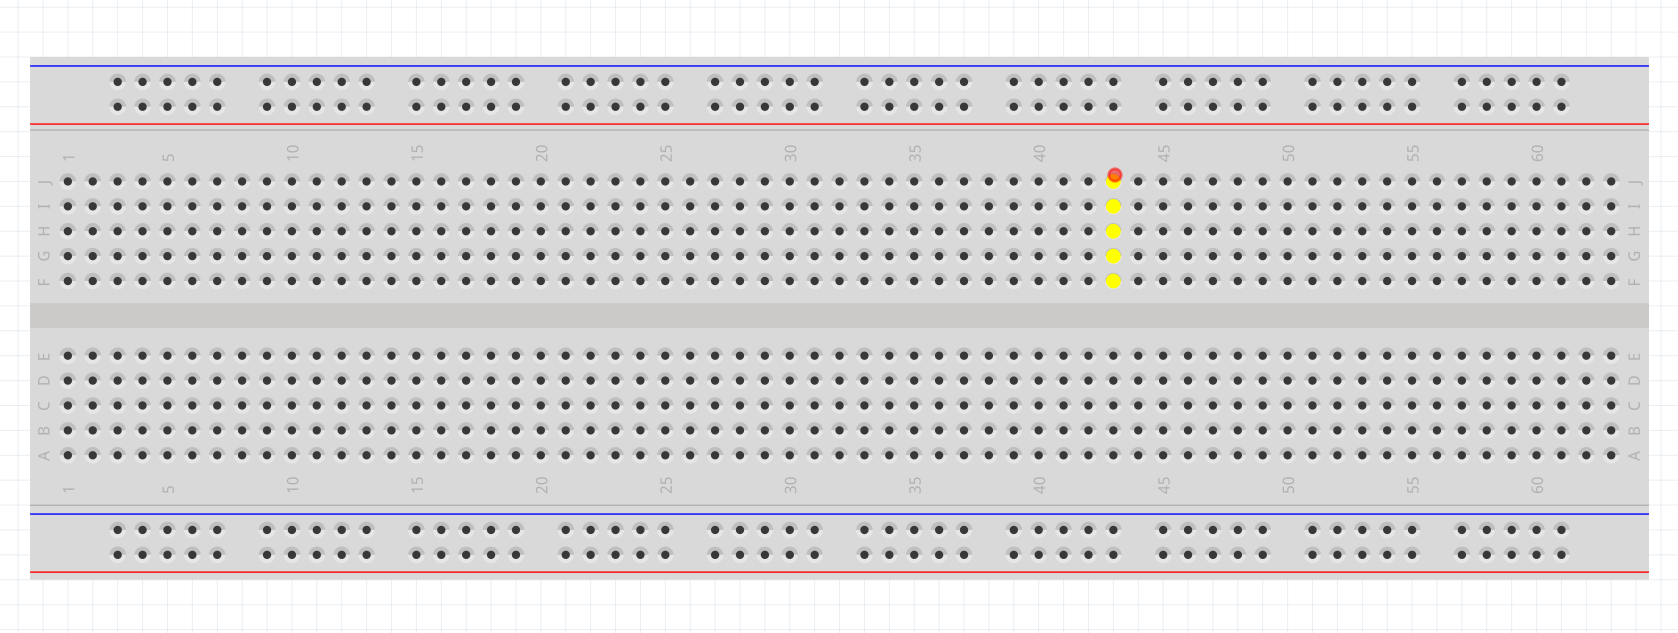
\includegraphics[width=0.9\textwidth]{images/Fritzing/breadboard2.png}
    \caption{ستون‌های عمودی پنج‌تایی}
    \label{fig:breadboard2}
\end{figure}

\begin{spacing}{1.3}
همانطور که در شکل \ref{fig:breadboard1} مشاهده می‌شود، چهار ردیف طولانی از ورودی‌ها، که به صورت دو جفت موازی در بالا و پایین بردبورد قرار دارند به هم متصل هستند. در شکل \ref{fig:breadboard2} نیز مشاهده می‌شود سایر وروری‌های بردبورد، به صورت گروه‌های پنج‌تایی 
عمودی به هم متصل می‌شوند.
\end{spacing}
	\subsection{مدار ساده \lr{LED}-مقاومت-باتری}
	\leavevmode\par
	\vspace{0.2cm}
	
	\begin{spacing}{1.3}
	پس از آشنایی با نحوه کار بردبورد، یک مدار ساده متشکل از یک عدد \lr{LED}، یک مقاومت و 
	باتری را با استفاده از آن می‌بندیم.
	\end{spacing}
	
	\pagebreak
	
\begin{center}
    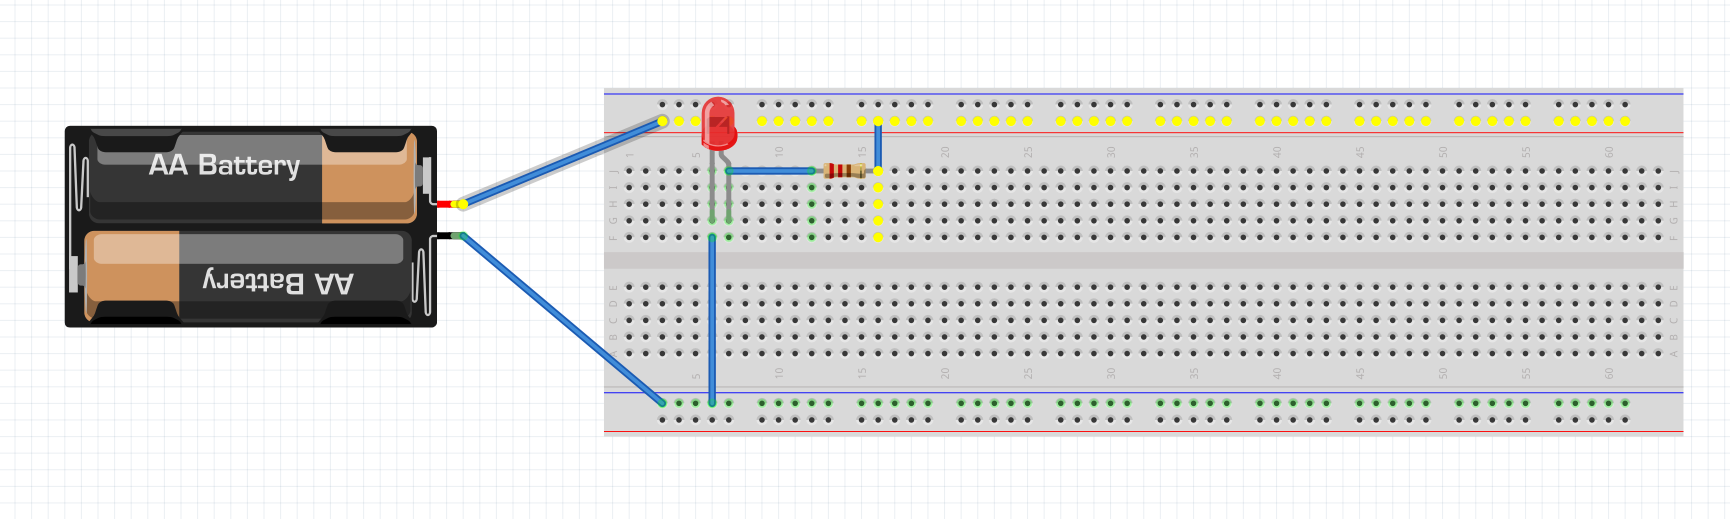
\includegraphics[width=0.9\textwidth]{images/Fritzing/led1.png}
    \captionof{figure}{}  % empty caption (or put a description)
    \label{fig:led1}
\end{center}

\begin{center}
    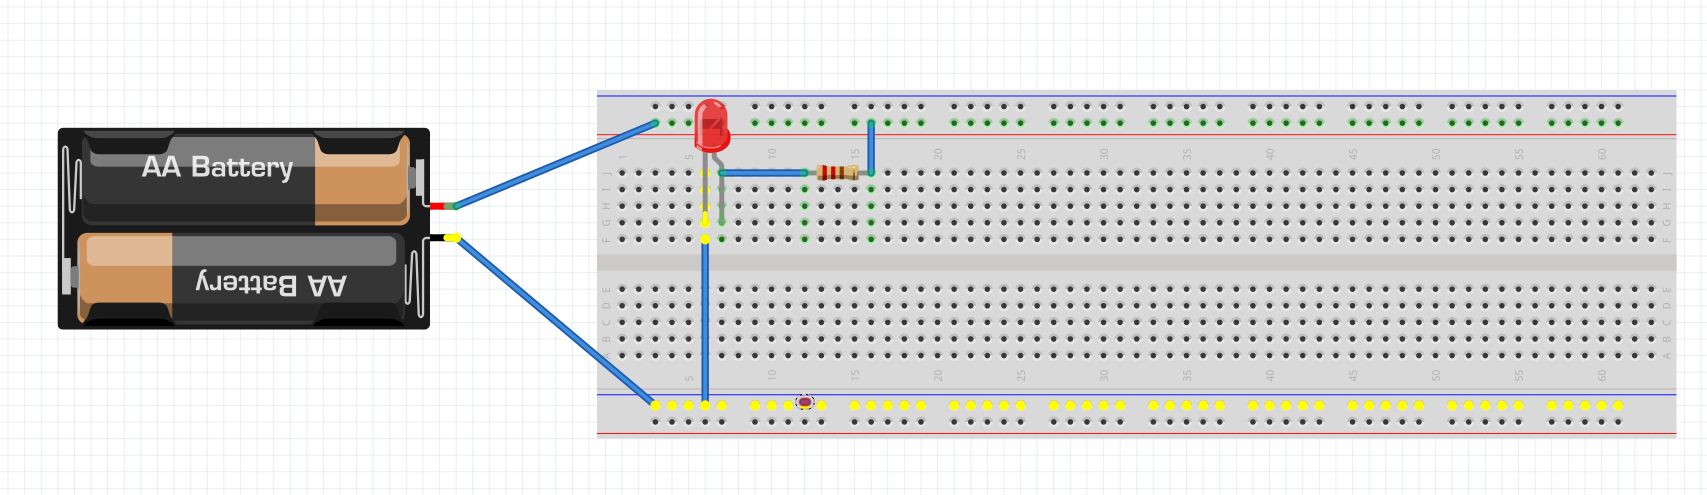
\includegraphics[width=0.9\textwidth]{images/Fritzing/led2.png}
    \captionof{figure}{}
    \label{fig:led2}
\end{center}

\begin{center}
    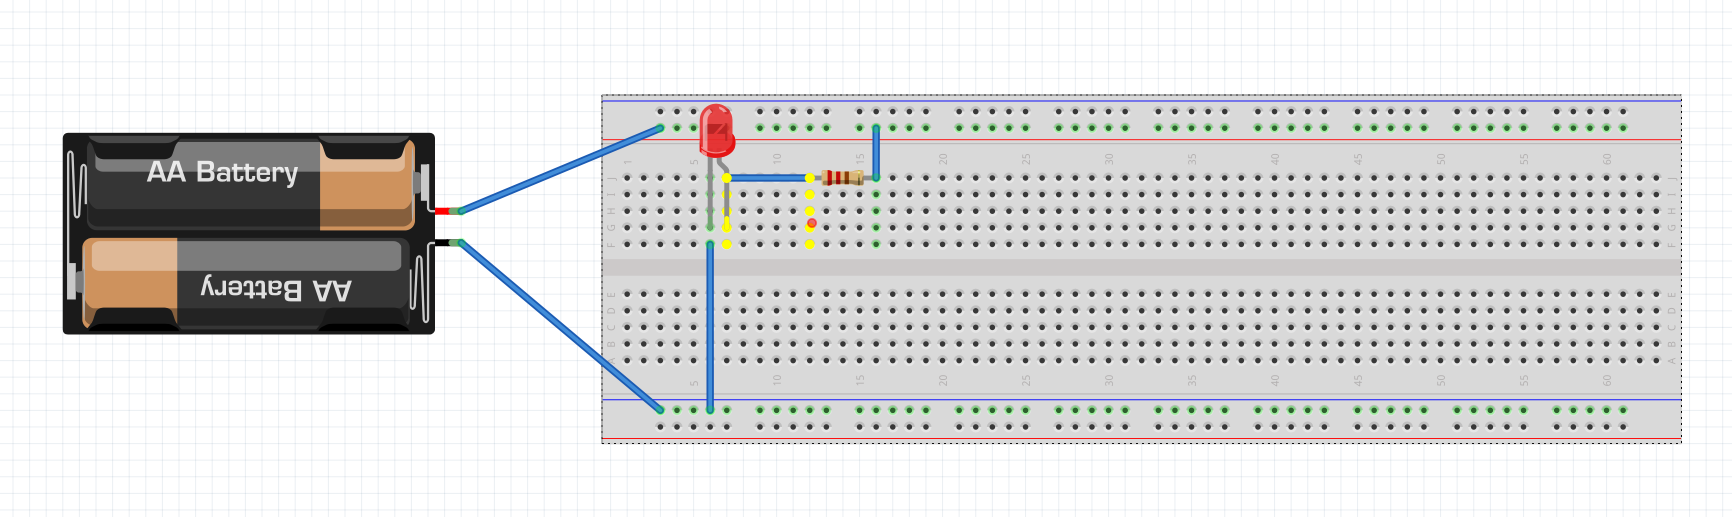
\includegraphics[width=0.9\textwidth]{images/Fritzing/led3.png}
    \captionof{figure}{}
    \label{fig:led3}
\end{center}

\begin{center}
    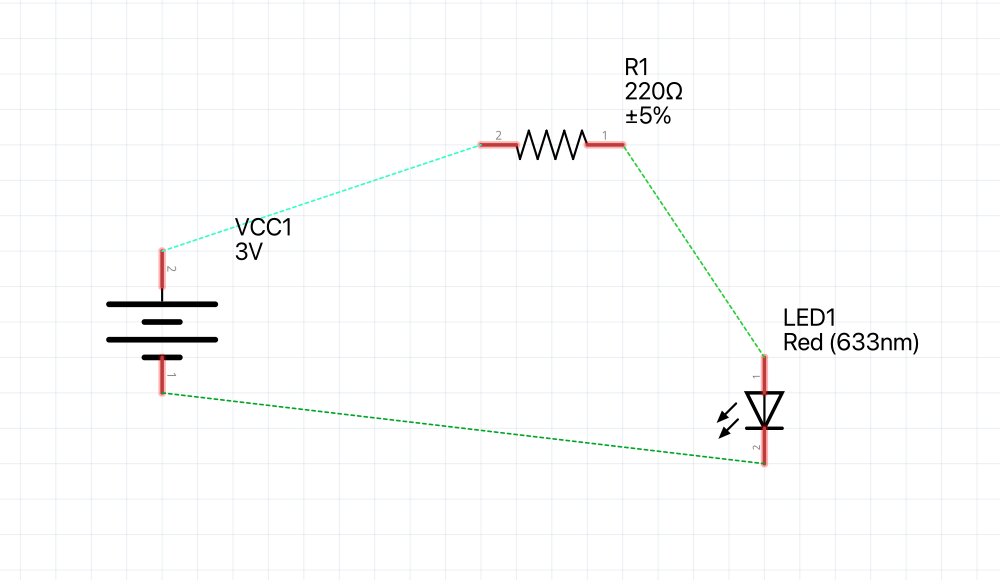
\includegraphics[width=0.7\textwidth]{images/Fritzing/led4.png}
    \captionof{figure}{}
    \label{fig:led4}
\end{center}
	
\begin{spacing}{1.3}
	در شکل های \ref{fig:led1} تا \ref{fig:led3} اتصالات قطعات نمایش داده شده‌است. معمولا از چهار ردیف افقی طولانی ورودی‌های متصل به هم به عنوان محل اتصال به منبع تغذیه(در اینجا باتری) استفاده می‌شود. علت وجود خطوط آبی و قرمز در کنار این ردیف ها نیز همین است.
\end{spacing}

\subsection{مدار تراشه 7404}
	\leavevmode\par
	\vspace{0.2cm}
	
\begin{minipage}{0.50\textwidth}          
    \begin{spacing}{1.3}
   خط افقی وسط بردبورد، که گروه های پنج‌تایی بالا و پایین را از هم جدا می‌کند، برای نصب \lr{IC} ها روی بردبورد استفاده می‌شود. اگر \lr{IC} را طور دیگری روی بردبورد ببندیم، بین پایه‌های آن اتصال کوتاه برقرار می‌شود.
    \end{spacing}
\end{minipage}%
\hfill%                                   
\begin{minipage}{0.4\textwidth}          
    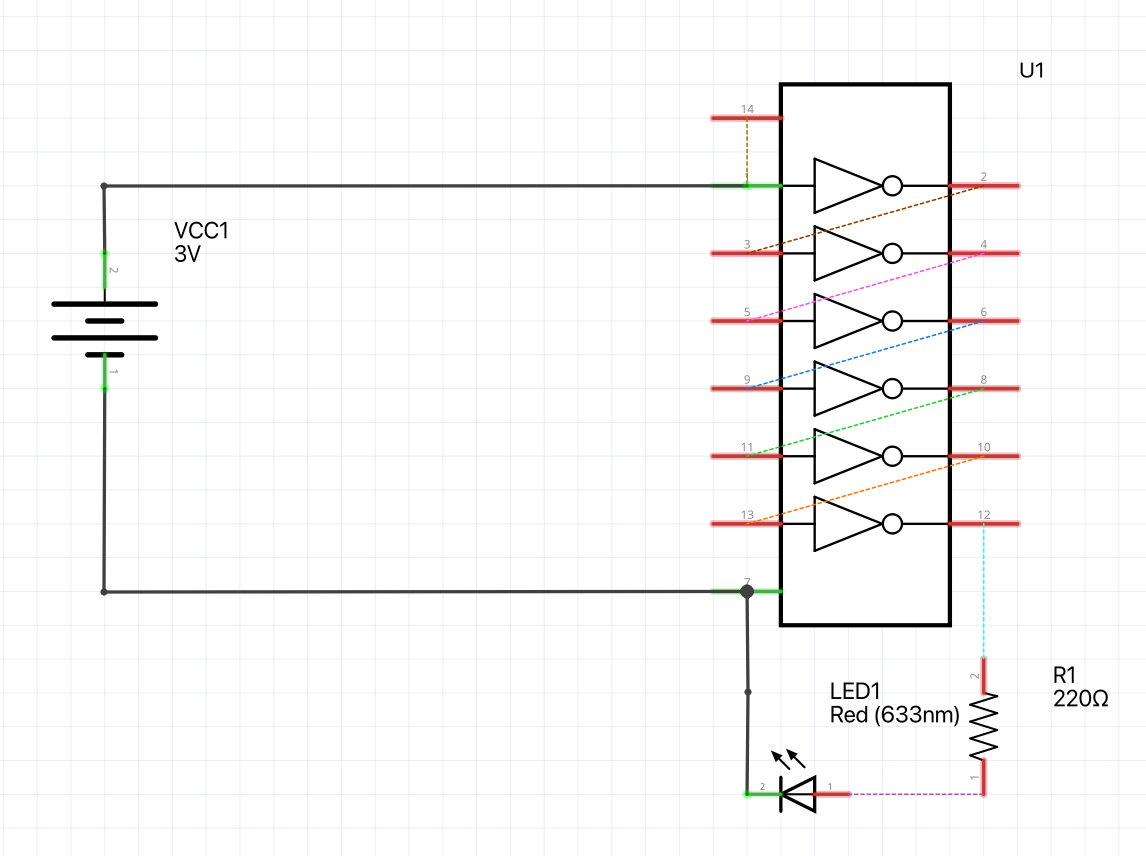
\includegraphics[width=\linewidth]{images/Fritzing/7404-1.png}
    \captionof{figure}{}
    \label{fig:7404-1}
\end{minipage}

\begin{figure}[htbp]                    
    \centering
    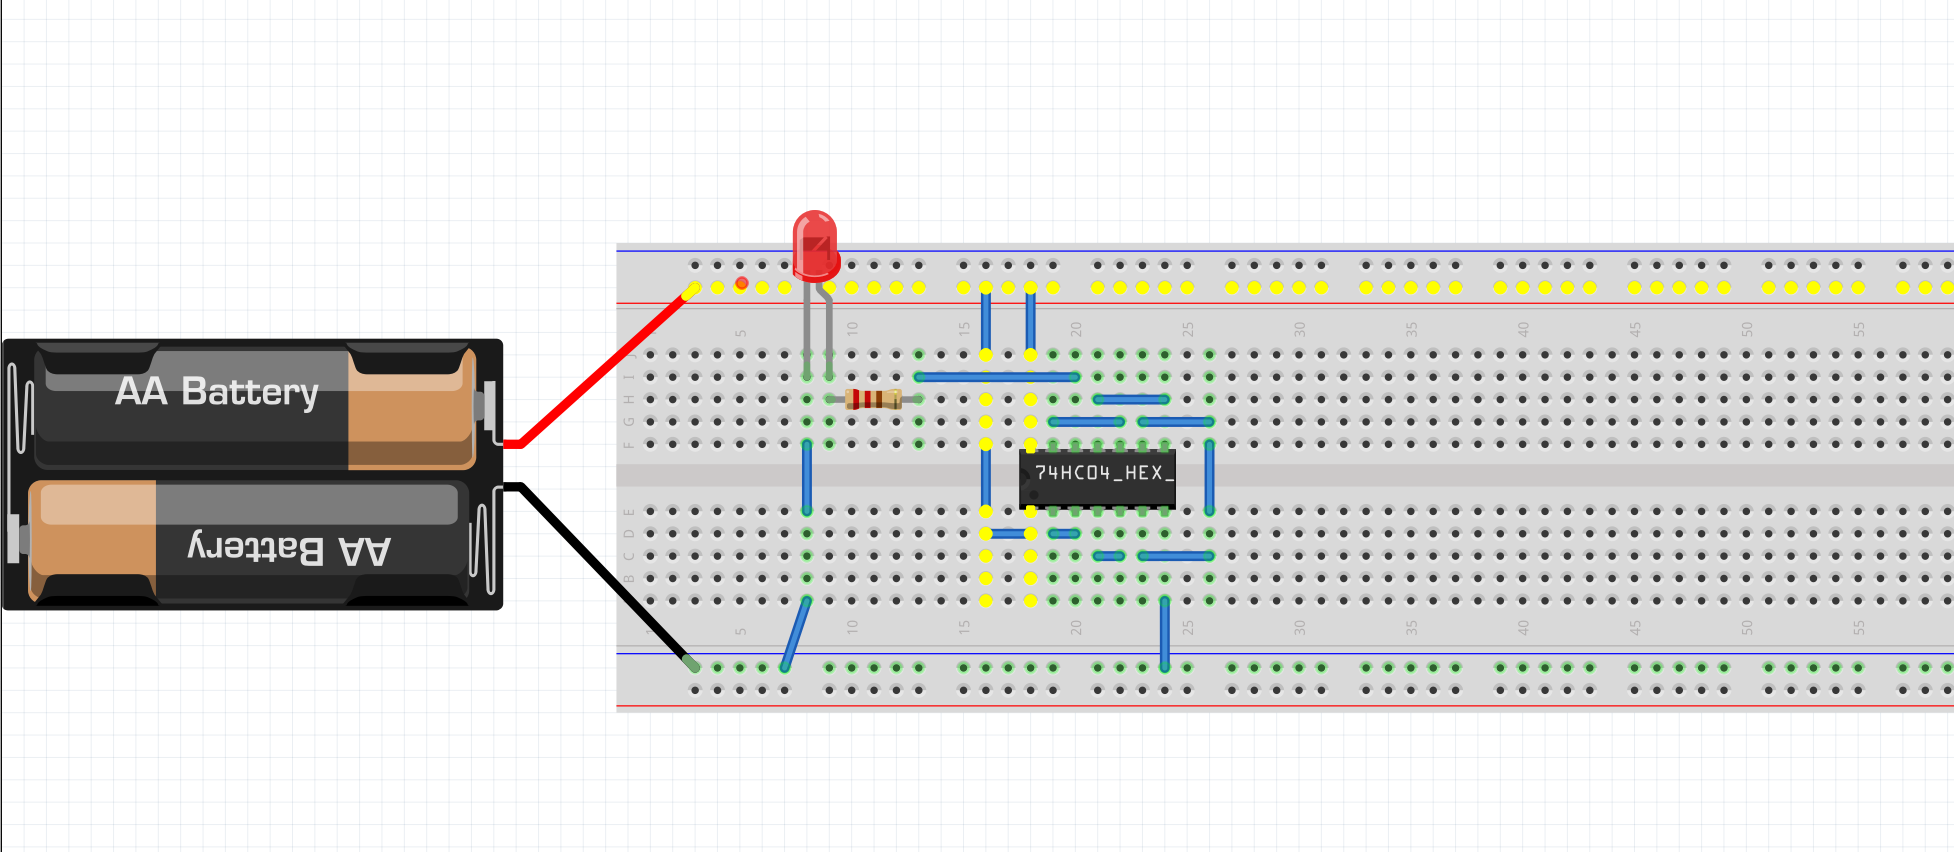
\includegraphics[width=0.9\textwidth]{images/Fritzing/7404-2.png}
    \caption{}      
    \label{fig:7404-2}
\end{figure}

    \begin{spacing}{1.3}
تراشه 7404 در واقع 6 گیت \rl{NOT} درون خود دارد که به جز پایه 7 و 14 که به ترتیب \rl{GND} و \rl{VCC} آن هستند، هر دو جفت پایه مجاور دیگر ورودی و خروجی یک گیت می‌باشند.
    \end{spacing}

\begin{figure}[htbp]                    
    \centering
    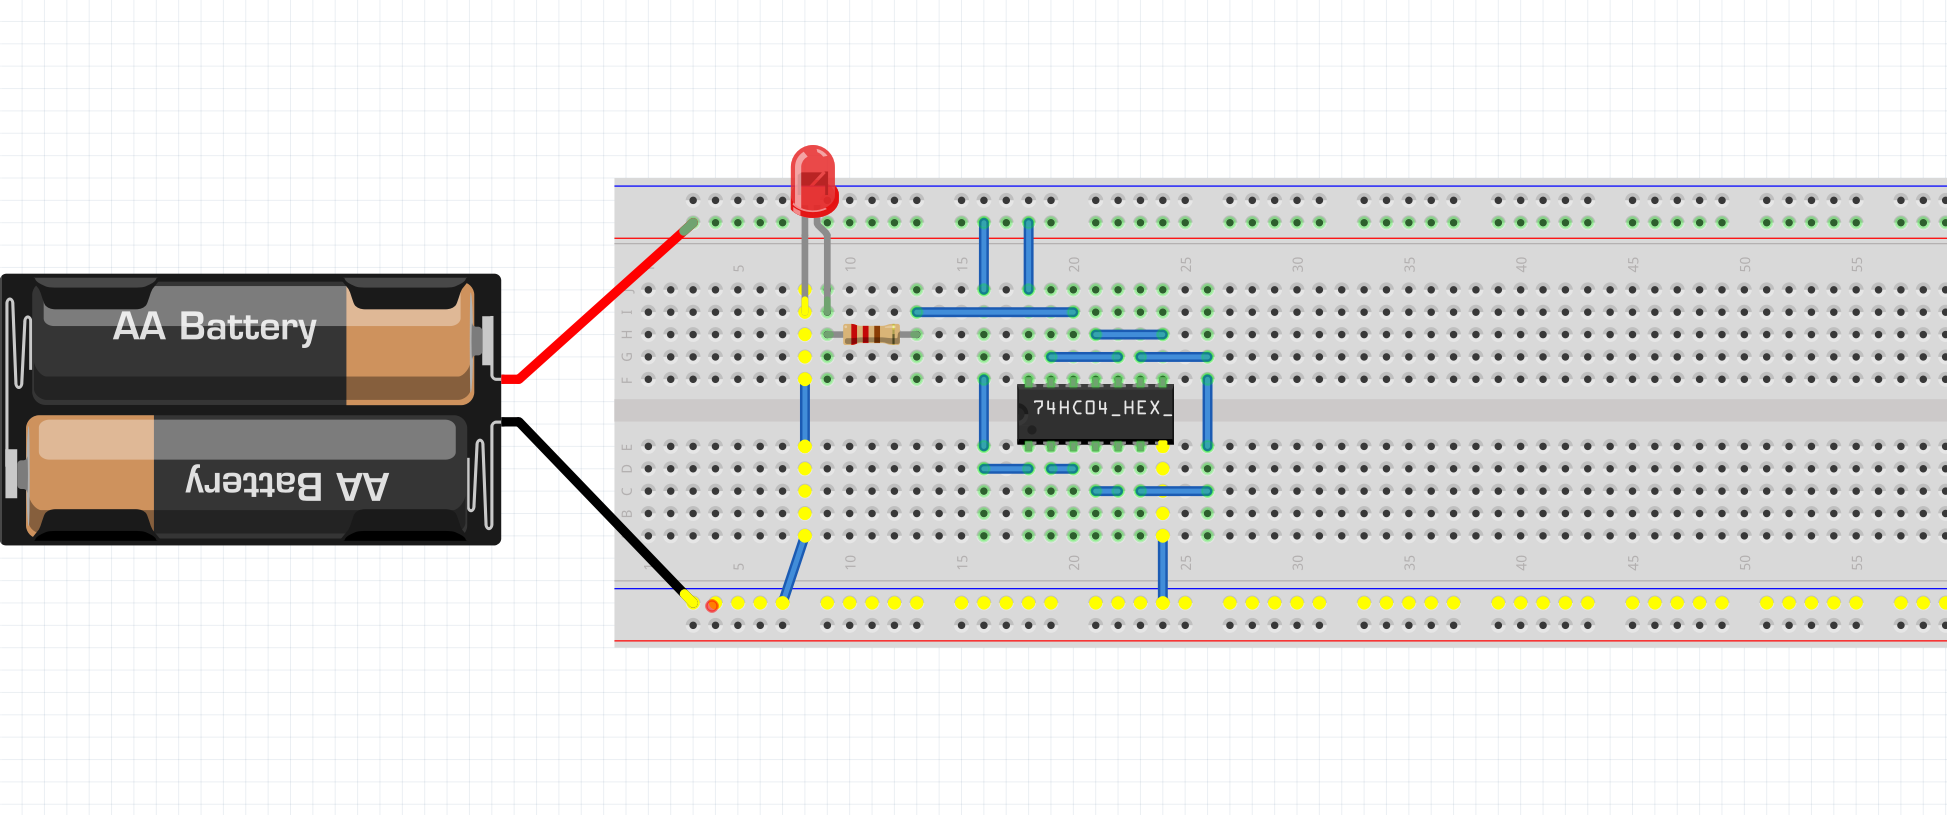
\includegraphics[width=0.9\textwidth]{images/Fritzing/7404-3.png}
    \caption{}      
    \label{fig:7404-3}
\end{figure}

\begin{figure}[htbp]                    
    \centering
    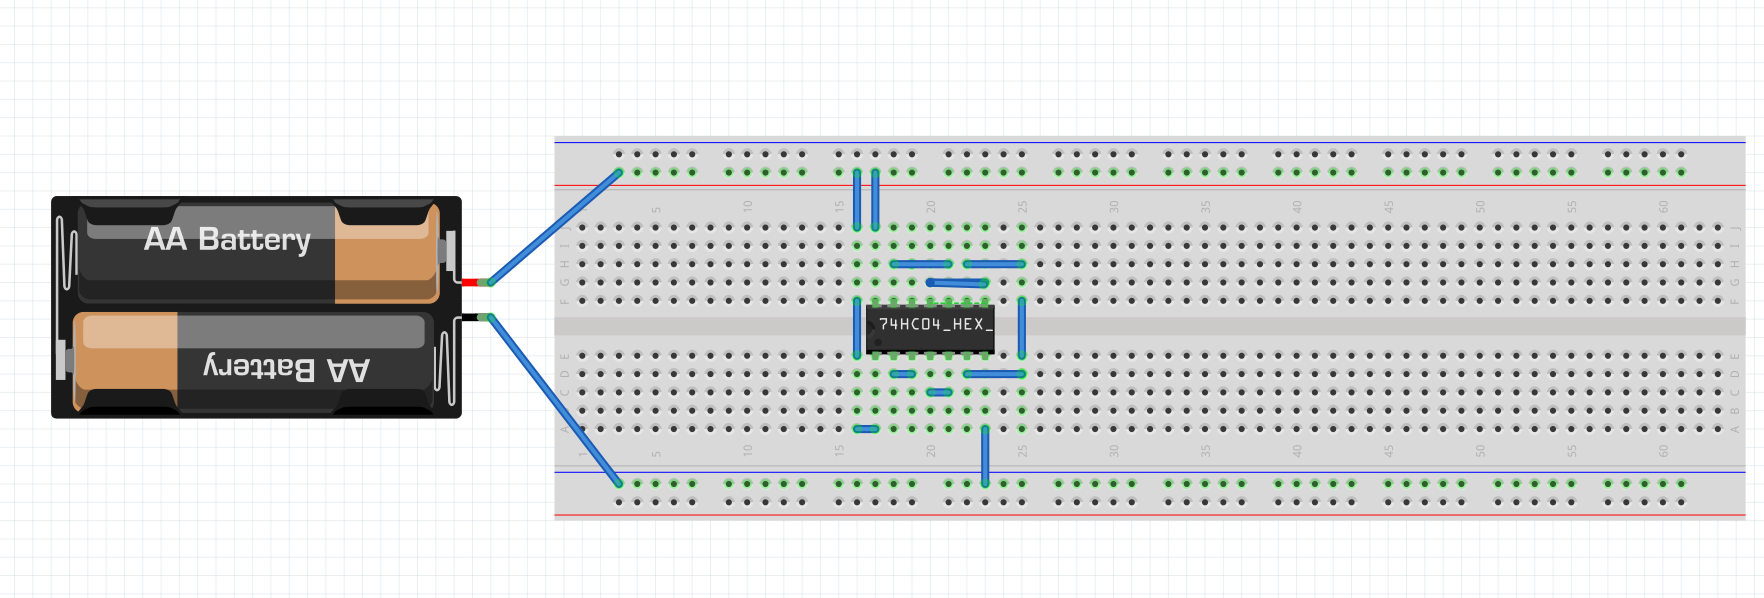
\includegraphics[width=0.9\textwidth]{images/Fritzing/7404-4.png}
    \caption{}      
    \label{fig:7404-4}
\end{figure}

\pagebreak

\section{ساخت مدار با \lr{Logisim}}
\leavevmode\par
\vspace{0.3cm}

\begin{spacing}{1.3}
در این قسمت با استفاده از نرم‌افزار \lr{Logisim} دو مدار ترکیبی می‌سازیم و تست می‌کنیم.
\end{spacing}

\subsection{مدار جمع‌کننده کامل(\lr{Full Adder})}
\label{subsec:fa}
\leavevmode\par
\vspace{0.2cm}

\begin{spacing}{1.3}
مدار جمع‌کننده کامل، سه ورودی \lr{$a$}، \lr{$b$} و \lr{$c_{in}$} را دریافت می‌کند و حاصل جمع آنها(\lr{$sum$}) و همچنین \lr{carry} تولید شده(\lr{$c_{out}$}) را خروجی می‌دهد. تصویر این مدار را در شکل \ref{fig:fa} مشاهده می‌کنید که با استفاده از گیت های \lr{AND}، \lr{OR} و \lr{XOR} ساخته شده‌است.
\end{spacing}

\begin{figure}[htbp]                     
    \centering
    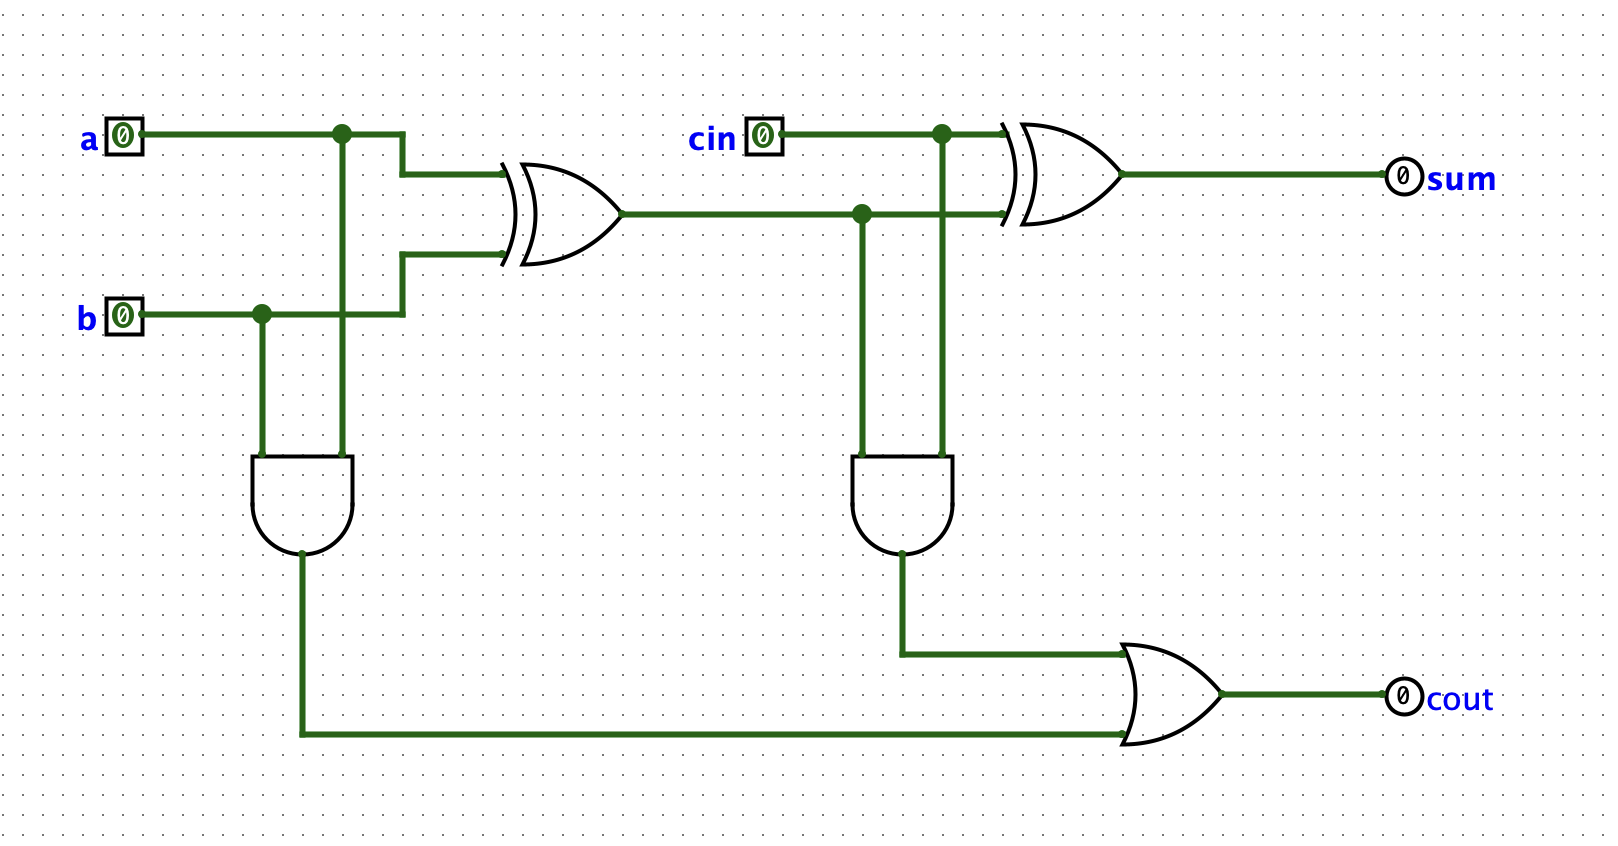
\includegraphics[width=0.9\textwidth]{images/Logisim/fa.png}
    \caption{مدار \lr{Full Adder}}       
    \label{fig:fa}
\end{figure}

\begin{figure}[htbp]                    
    \centering
    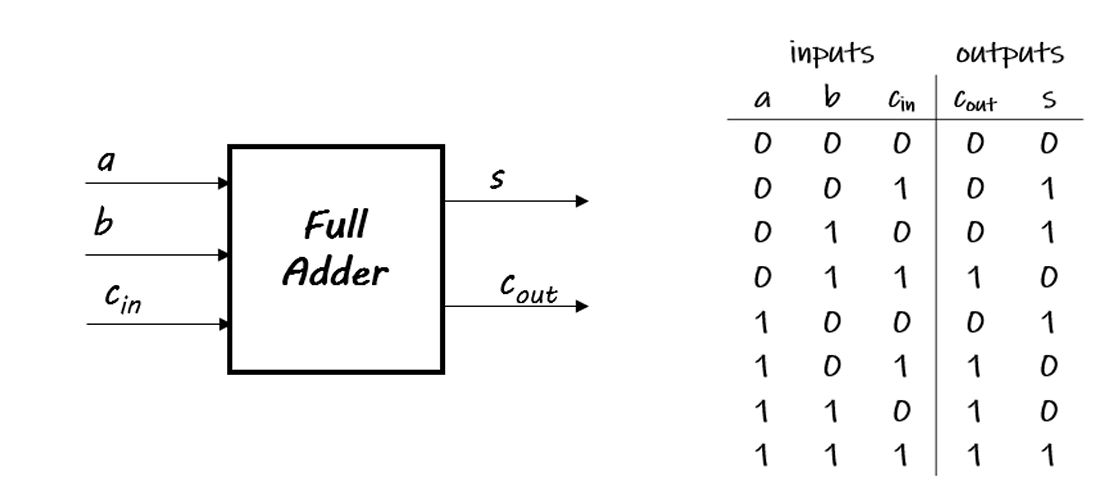
\includegraphics[width=0.9\textwidth]{images/Logisim/fa2.png}
    \caption{}       
    \label{fig:fa2}
\end{figure}

\subsection{مدار جمع‌کننده/تفریق‌کننده چهاربیتی}
\leavevmode\par
\vspace{0.2cm}

\begin{spacing}{1.3}
حال با استفاده از چهار مدار جمع‌کننده کامل که در بخش \ref{subsec:fa} ساختیم، یک مدار جمع‌کننده/تفریق‌کننده\LTRfootnote{Adder/Subtractor} می‌سازیم که اگر مقدار ورودی \lr{$c_{in}$} صفر باشد، حاصل جمع و در غیر این صورت، حاصل تفریق دو ورودی چهاربیتی را تولید کند.
\end{spacing}

\begin{figure}[htbp]                    
    \centering
    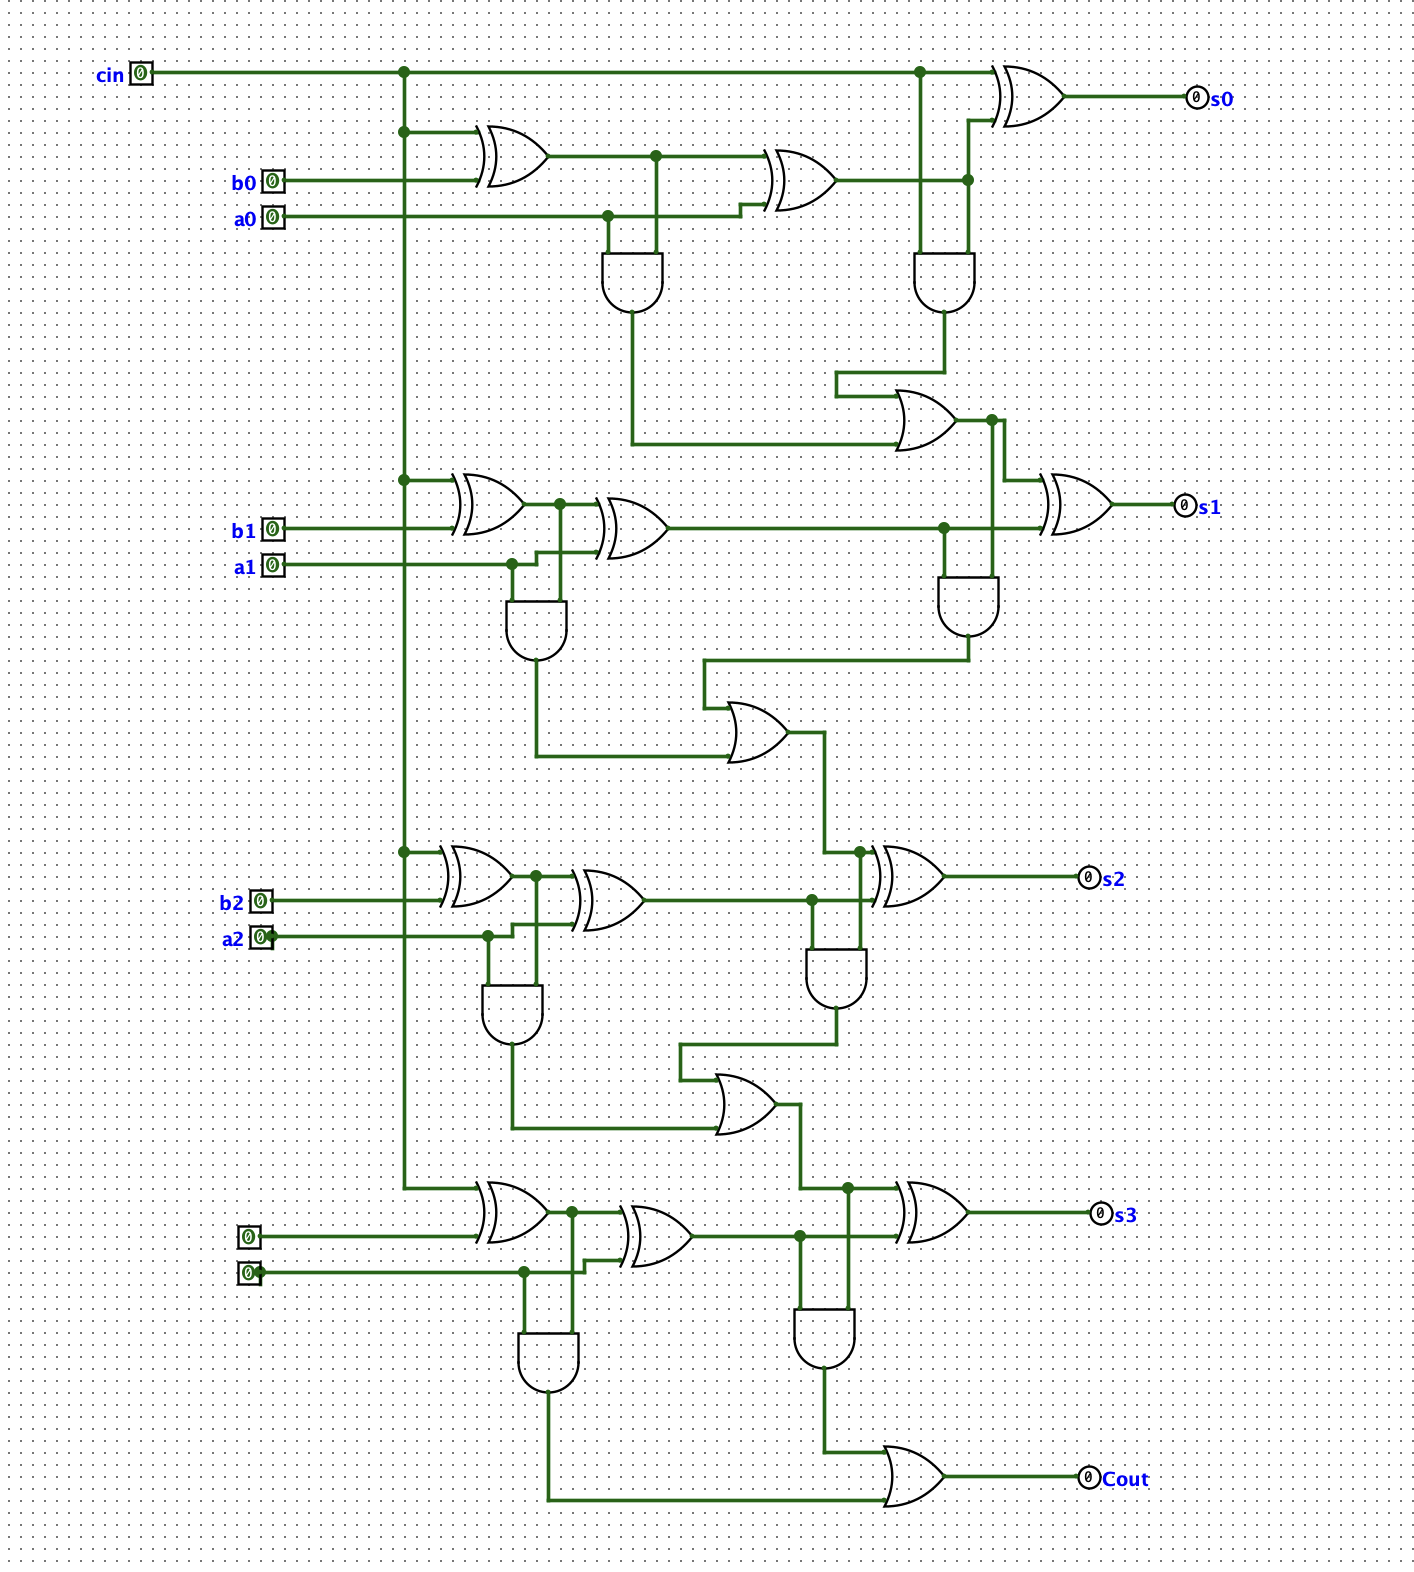
\includegraphics[width=0.9\textwidth]{images/Logisim/as1.png}
    \caption{}       
    \label{fig:as1}
\end{figure}

\begin{spacing}{1.3}
عملکرد مدار شکل \ref{fig:as1} به این صورت است که اگر \lr{$c_{in} = 0$} گیت‌های \lr{XOR} که یک ورودی آنها بیت های \lr{$B$} است، آن بیت را بدون تغییر به \lr{Full Adder} می‌فرستند تا با بیت متناظر از \lr{$A$} جمع شود.

اما اگر \lr{$c_{in} = 0$}، گیت‌های \lr{XOR} تمام بیت‌های \lr{$B$} را \lr{NOT} می‌کنند و در نهایت عددی که با \lr{$A$} جمع می‌شود، \lr{$\overline{B}$} خواهد بود. با در نظر گرفتن ورودی \lr{$c_{in} = 1$}، در نهایت خروجی محاسبه شده توسط مدار، \lr{$A + \overline{B} + 1$} است که در آن \lr{$\overline{B} + 1$}، مکمل دو\LTRfootnote{2's complement} \lr{$B$} می‌باشد. یعنی مدار در نهایت \lr{$A-B$} را محاسبه می‌کند.
\lr{$$ A + \overline{B} + 1 = A + \text{2's-complement}(B) = A-B $$}
\end{spacing}


\begin{figure}[htbp]                    
    \centering
    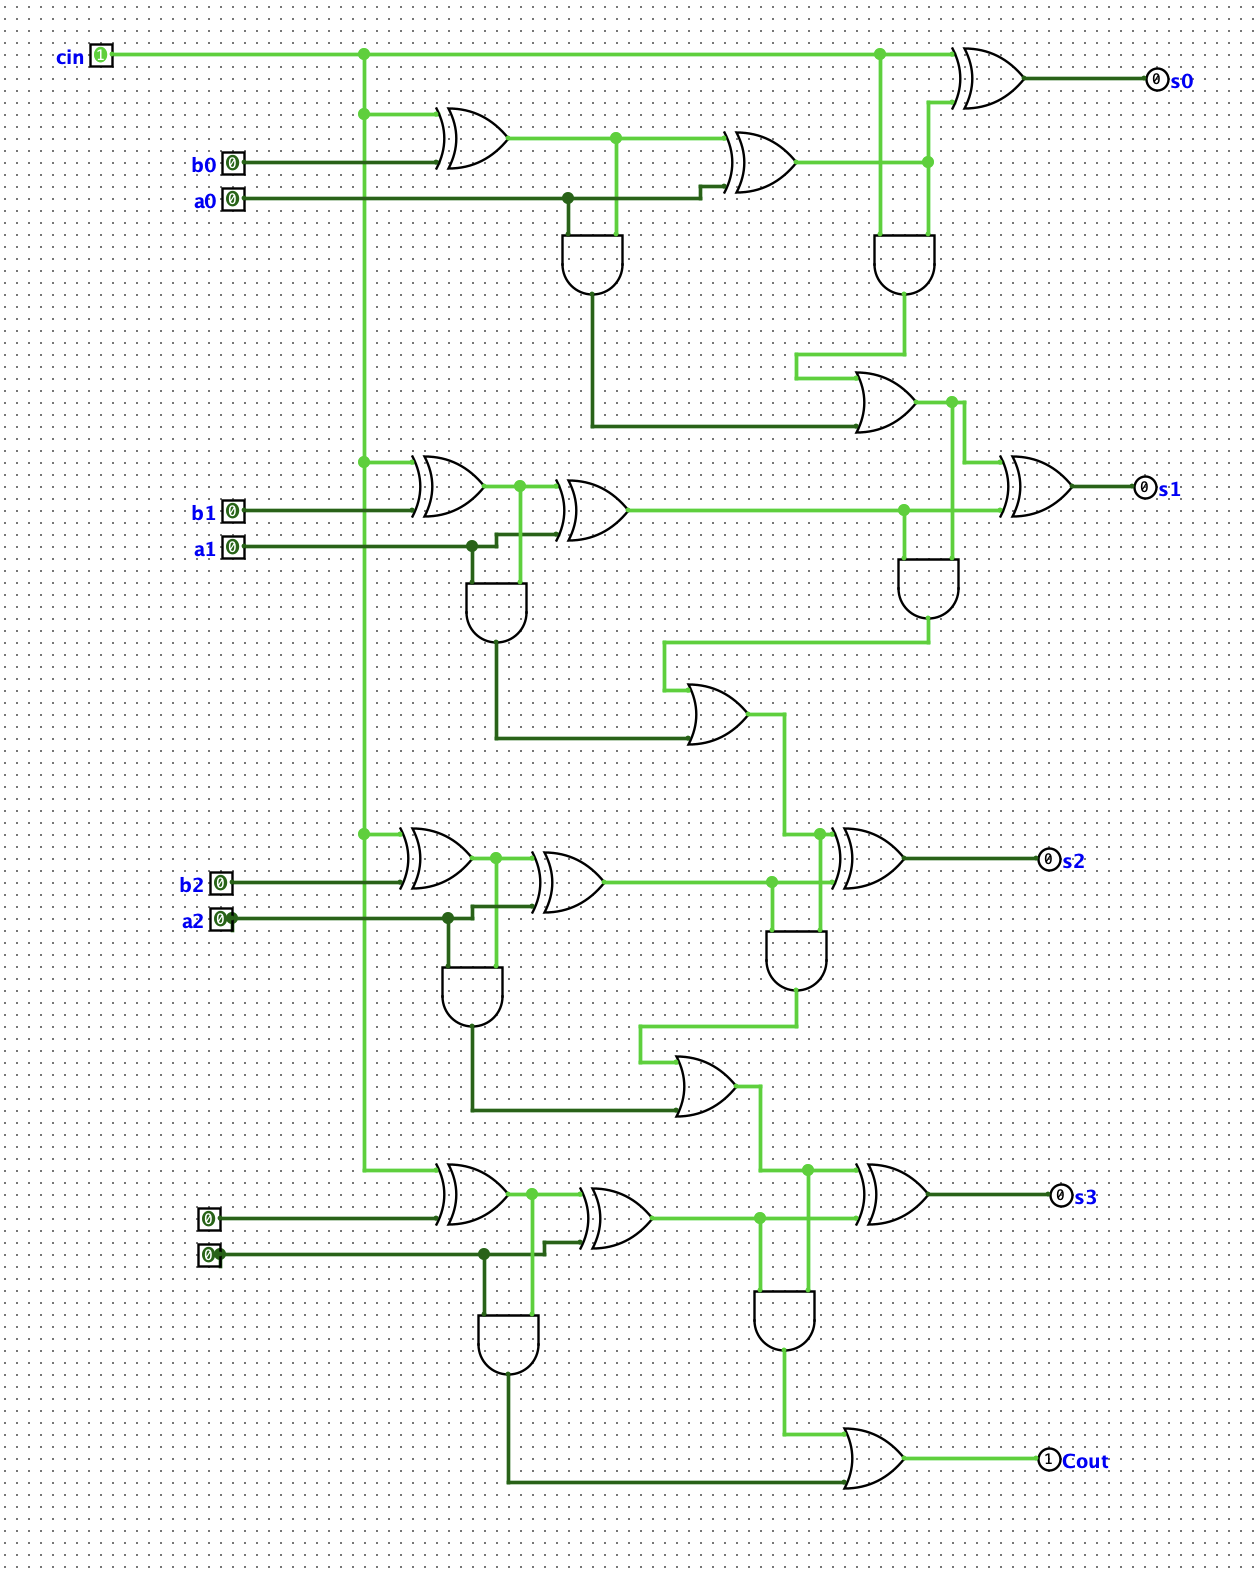
\includegraphics[width=0.8\textwidth]{images/Logisim/as2.png}
    \caption{}       
    \label{fig:as2}
\end{figure}

\begin{figure}[htbp]                    
    \centering
    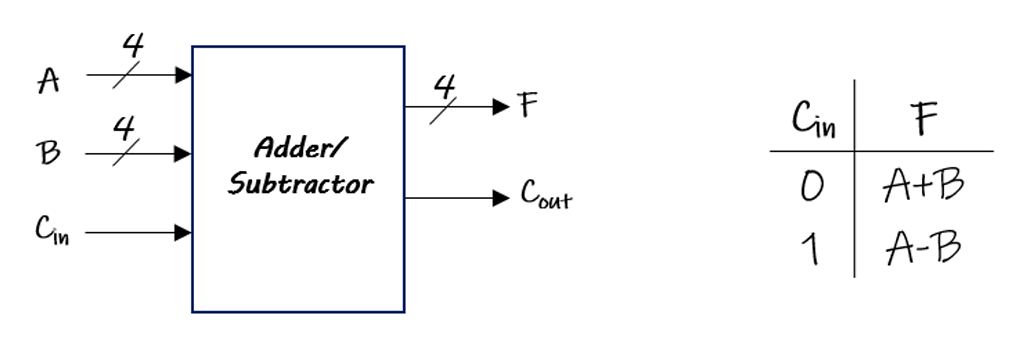
\includegraphics[width=0.9\textwidth]{images/Logisim/as3.png}
    \caption{}       
    \label{fig:as3}
\end{figure}

\subsection{تست مدارها}
\leavevmode\par
\vspace{0.2cm}

\subsubsection*{تست مدار \lr{Full Adder}}
\leavevmode\par
\vspace{0.2cm}

\begin{spacing}{1.3}
در تمام تست‌های \ref{fig:fat1} تا \ref{fig:fat7}، خروجی مدار با جدول \ref{fig:fa2} تطابق دارد.
\end{spacing}

\begin{figure}[htbp]                    
    \centering
    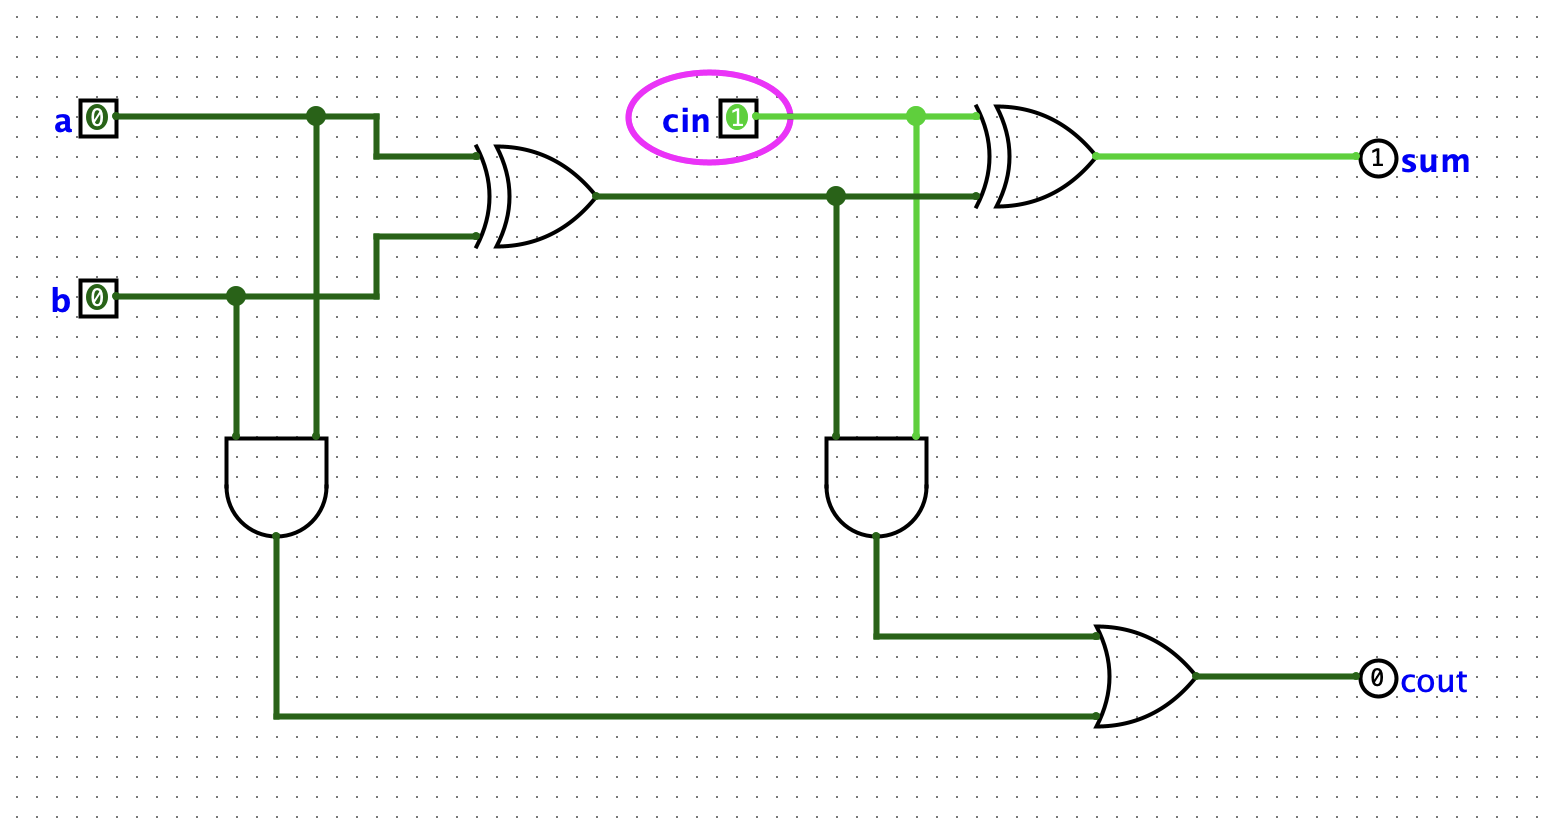
\includegraphics[width=0.7\textwidth]{images/Logisim/fat1.png}
    \caption{}       
    \label{fig:fat1}
\end{figure}

\begin{figure}[htbp]                    
    \centering
    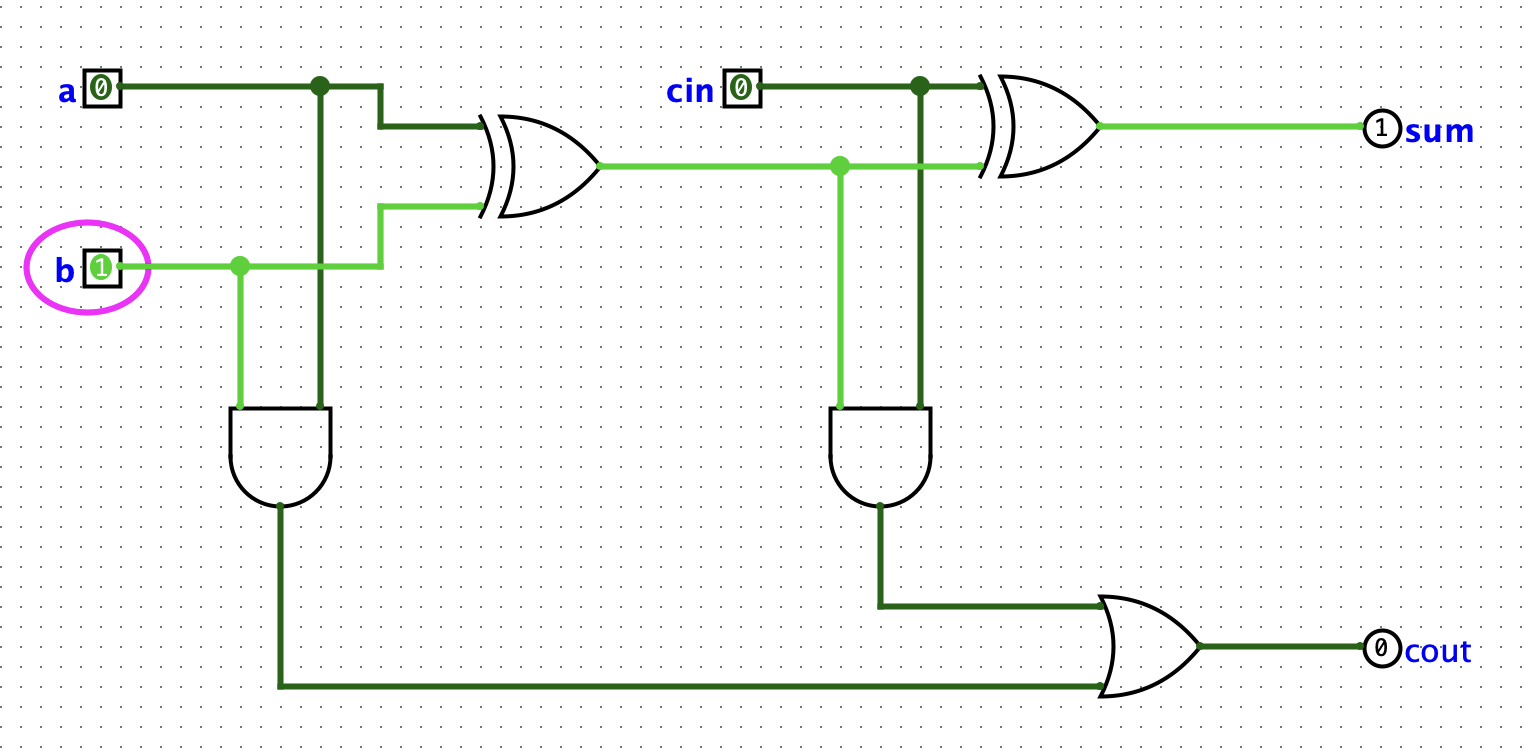
\includegraphics[width=0.7\textwidth]{images/Logisim/fat2.png}
    \caption{}       
    \label{fig:fat2}
\end{figure}

\begin{figure}[htbp]                    
    \centering
    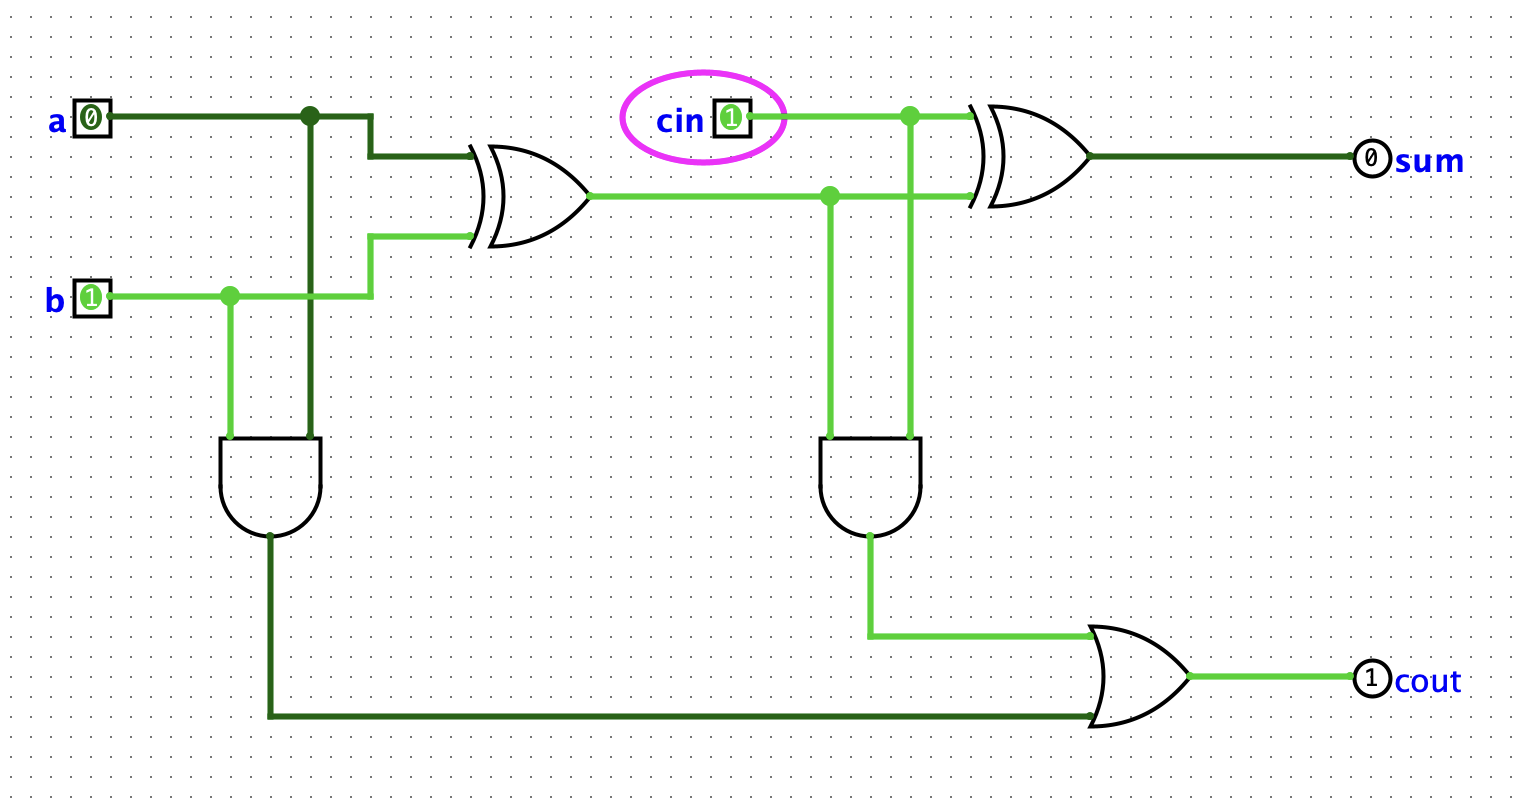
\includegraphics[width=0.7\textwidth]{images/Logisim/fat3.png}
    \caption{}       
    \label{fig:fat3}
\end{figure}

\begin{figure}[htbp]                    
    \centering
    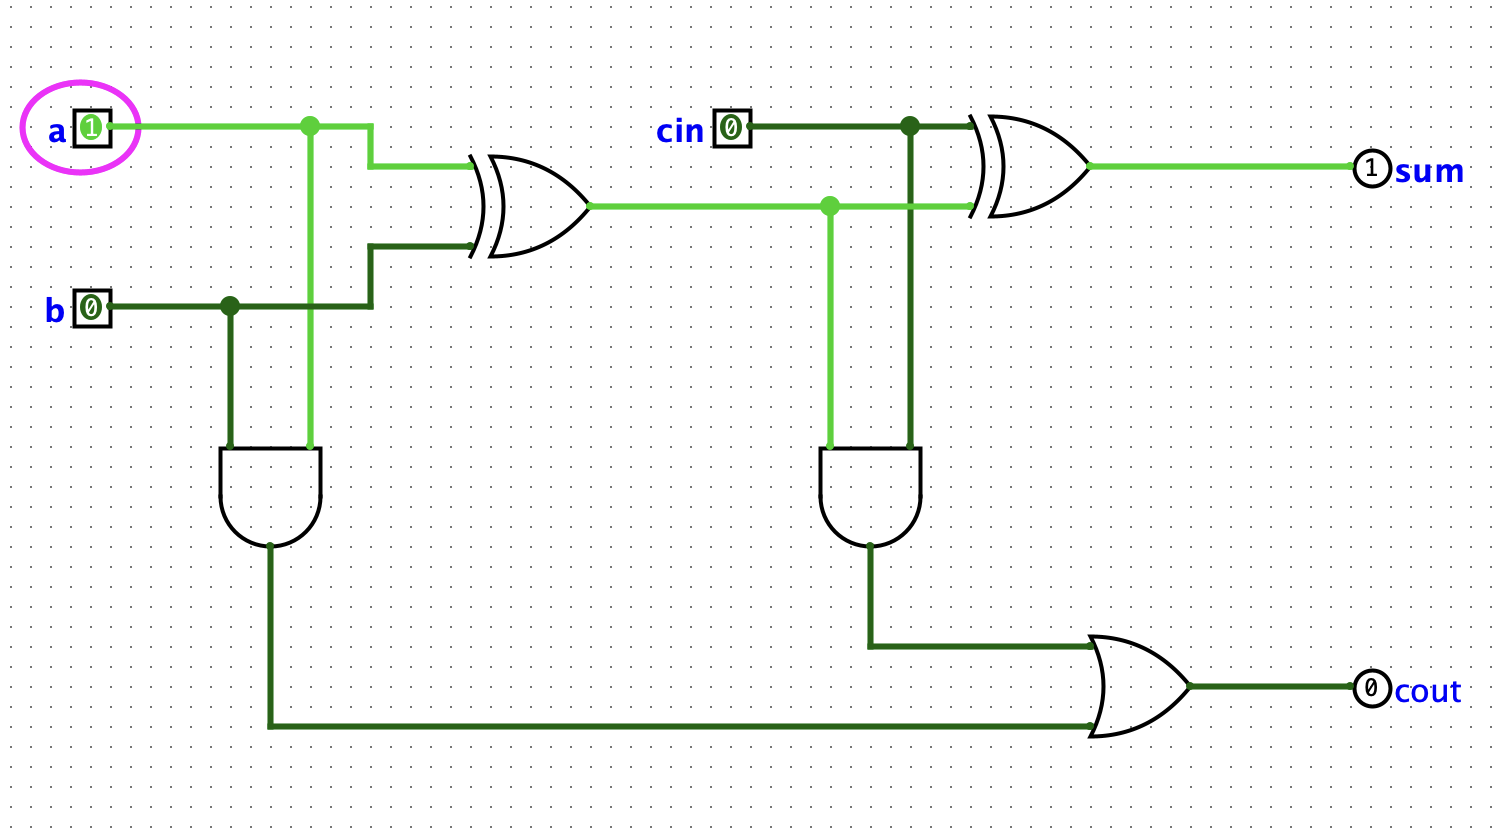
\includegraphics[width=0.7\textwidth]{images/Logisim/fat4.png}
    \caption{}       
    \label{fig:fat4}
\end{figure}

\begin{figure}[htbp]                    
    \centering
    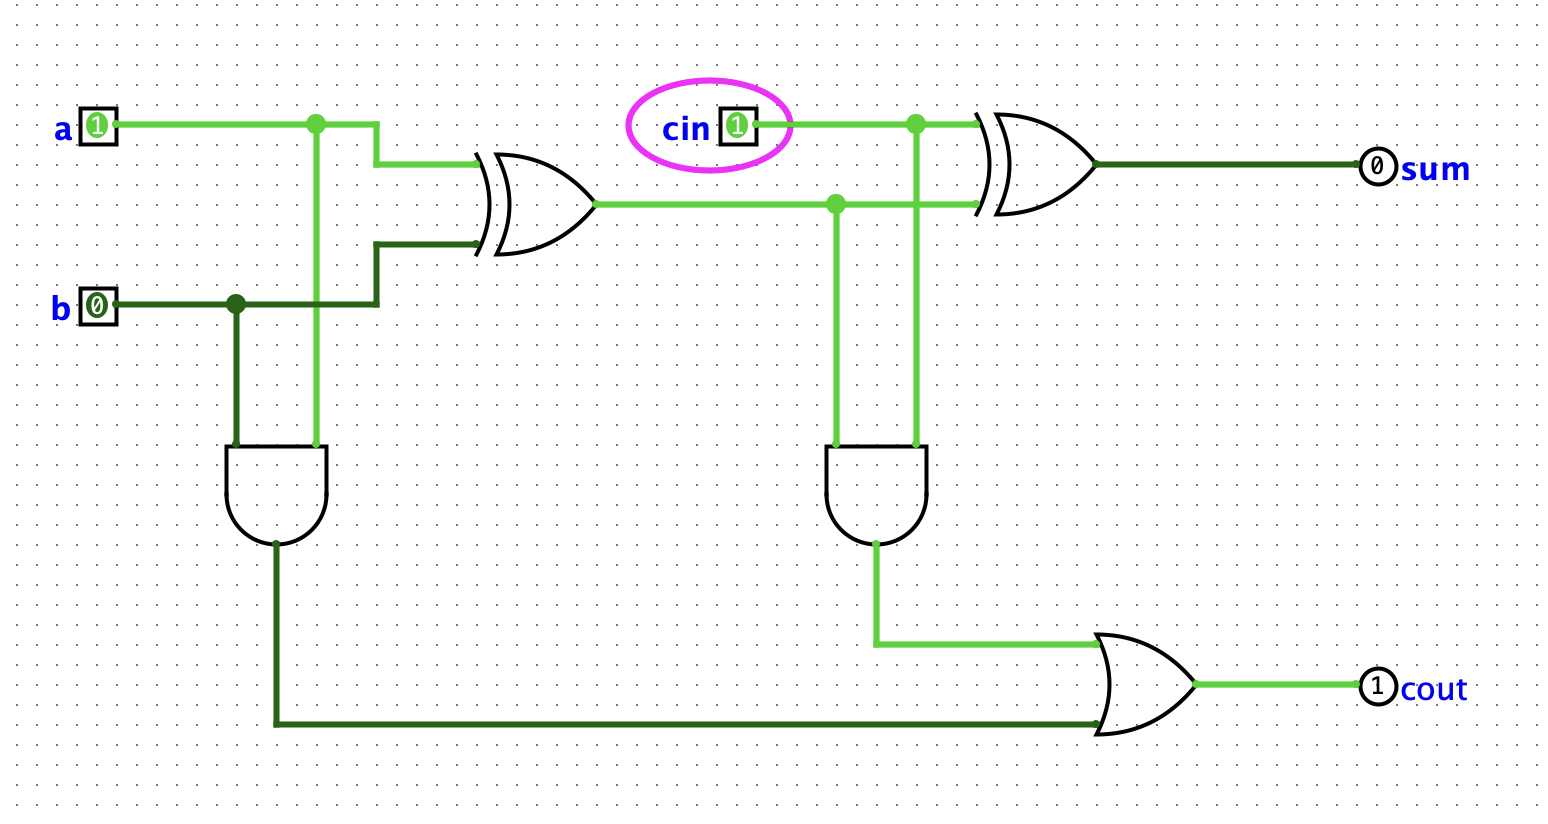
\includegraphics[width=0.7\textwidth]{images/Logisim/fat5.png}
    \caption{}       
    \label{fig:fat5}
\end{figure}

\begin{figure}[htbp]                    
    \centering
    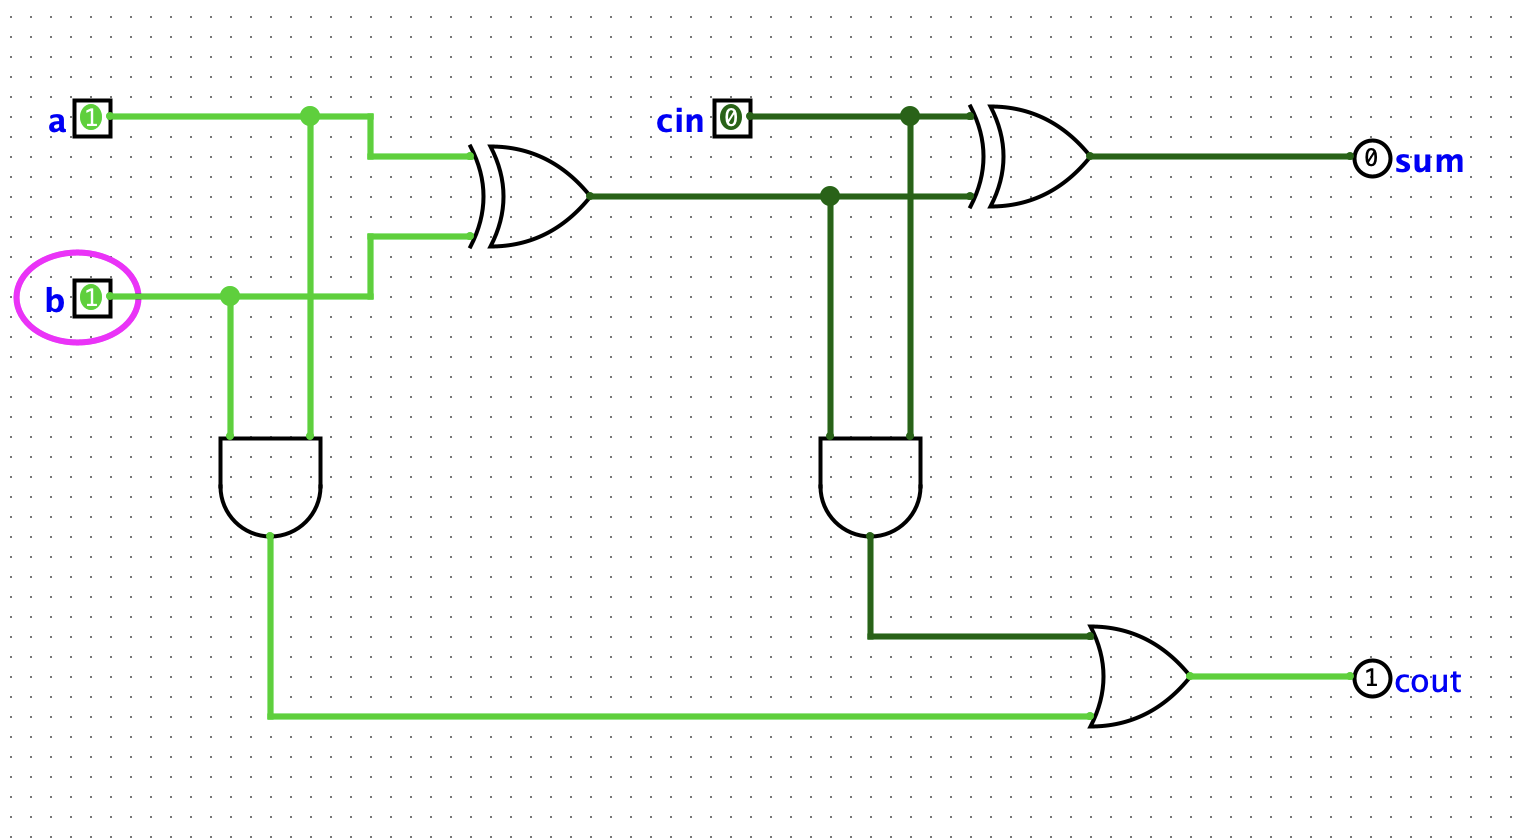
\includegraphics[width=0.7\textwidth]{images/Logisim/fat6.png}
    \caption{}       
    \label{fig:fat6}
\end{figure}

\begin{figure}[htbp]                    
    \centering
    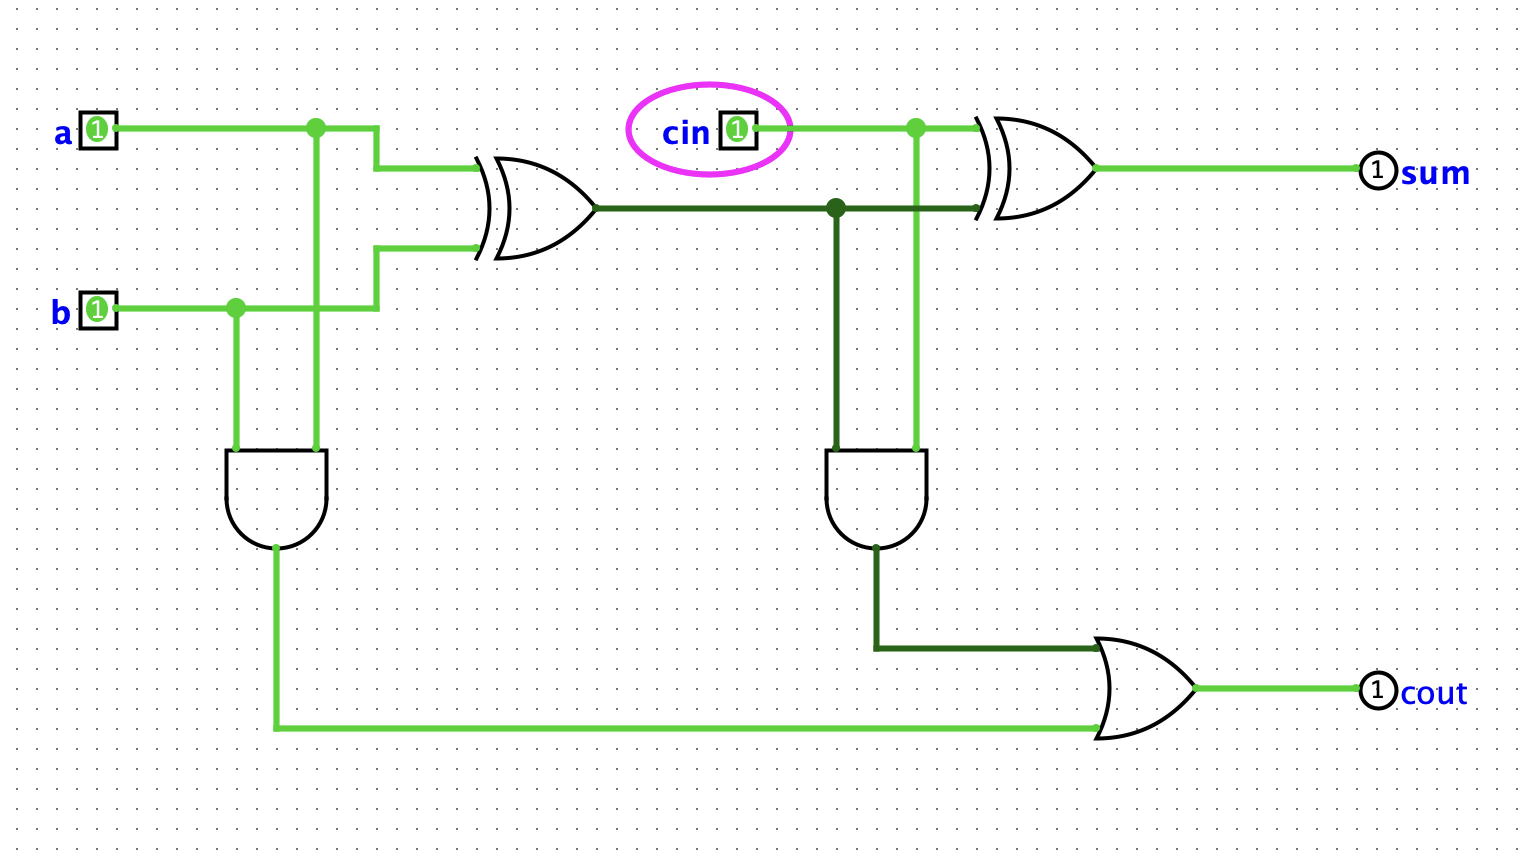
\includegraphics[width=0.7\textwidth]{images/Logisim/fat7.png}
    \caption{}       
    \label{fig:fat7}
\end{figure}

\pagebreak

\subsubsection*{تست مدار جمع‌کننده/تفریق‌کننده}
\leavevmode\par
\vspace{0.2cm}

\begin{spacing}{1.3}
شکل \ref{fig:ast1}:

\begin{latin}
$c_{in} = 0 \to$ addition

binary: $(1111)_2 + (0100)_2 = (10011)_2$

decimal: $15 + 4 = 19$
\end{latin}

شکل \ref{fig:ast2}:

\begin{latin}
$c_{in} = 0 \to$ addition

binary: $(0111)_2 + (0010)_2 = (01001)_2$

decimal: $7 + 2 = 9$
\end{latin}

شکل \ref{fig:ast3}:

\begin{latin}
$c_{in} = 0 \to$ addition

binary: $(1111)_2 + (1111)_2 = (11110)_2$

decimal: $15 + 15 = 30$
\end{latin}

شکل \ref{fig:ast4}:

\begin{latin}
$c_{in} = 1 \to$ subtraction

binary: $(1000)_2 - (0110)_2 = (0010)_2$

decimal: $8 - 6 = 2$
\end{latin}

شکل \ref{fig:ast5}:

\begin{latin}
$c_{in} = 1 \to$ subtraction

binary: $(0000)_2 - (0101)_2 = (1011)_2$

decimal: $0 - 5 = -5$
\end{latin}

توجه کنید که در سیستم مکمل دو، \lr{MSB} نمایانگر علامت است و در اینجا جواب ما عددی منفی است. برای بدست آوردن اندازه جواب از آن مکمل دو می‌گیریم.

شکل \ref{fig:ast6}:

\begin{latin}
$c_{in} = 1 \to$ subtraction

binary: $(0111)_2 - (1000)_2 = (1111)_2$

decimal: $7 - 8 = -1$
\end{latin}

شکل \ref{fig:ast7}:

\begin{latin}
$c_{in} = 1 \to$ subtraction

binary: $(0100)_2 - (0010)_2 = (0010)_2$

decimal: $4 - 2 = 2$
\end{latin}


\end{spacing}

\begin{figure}[htbp]                    
    \centering
    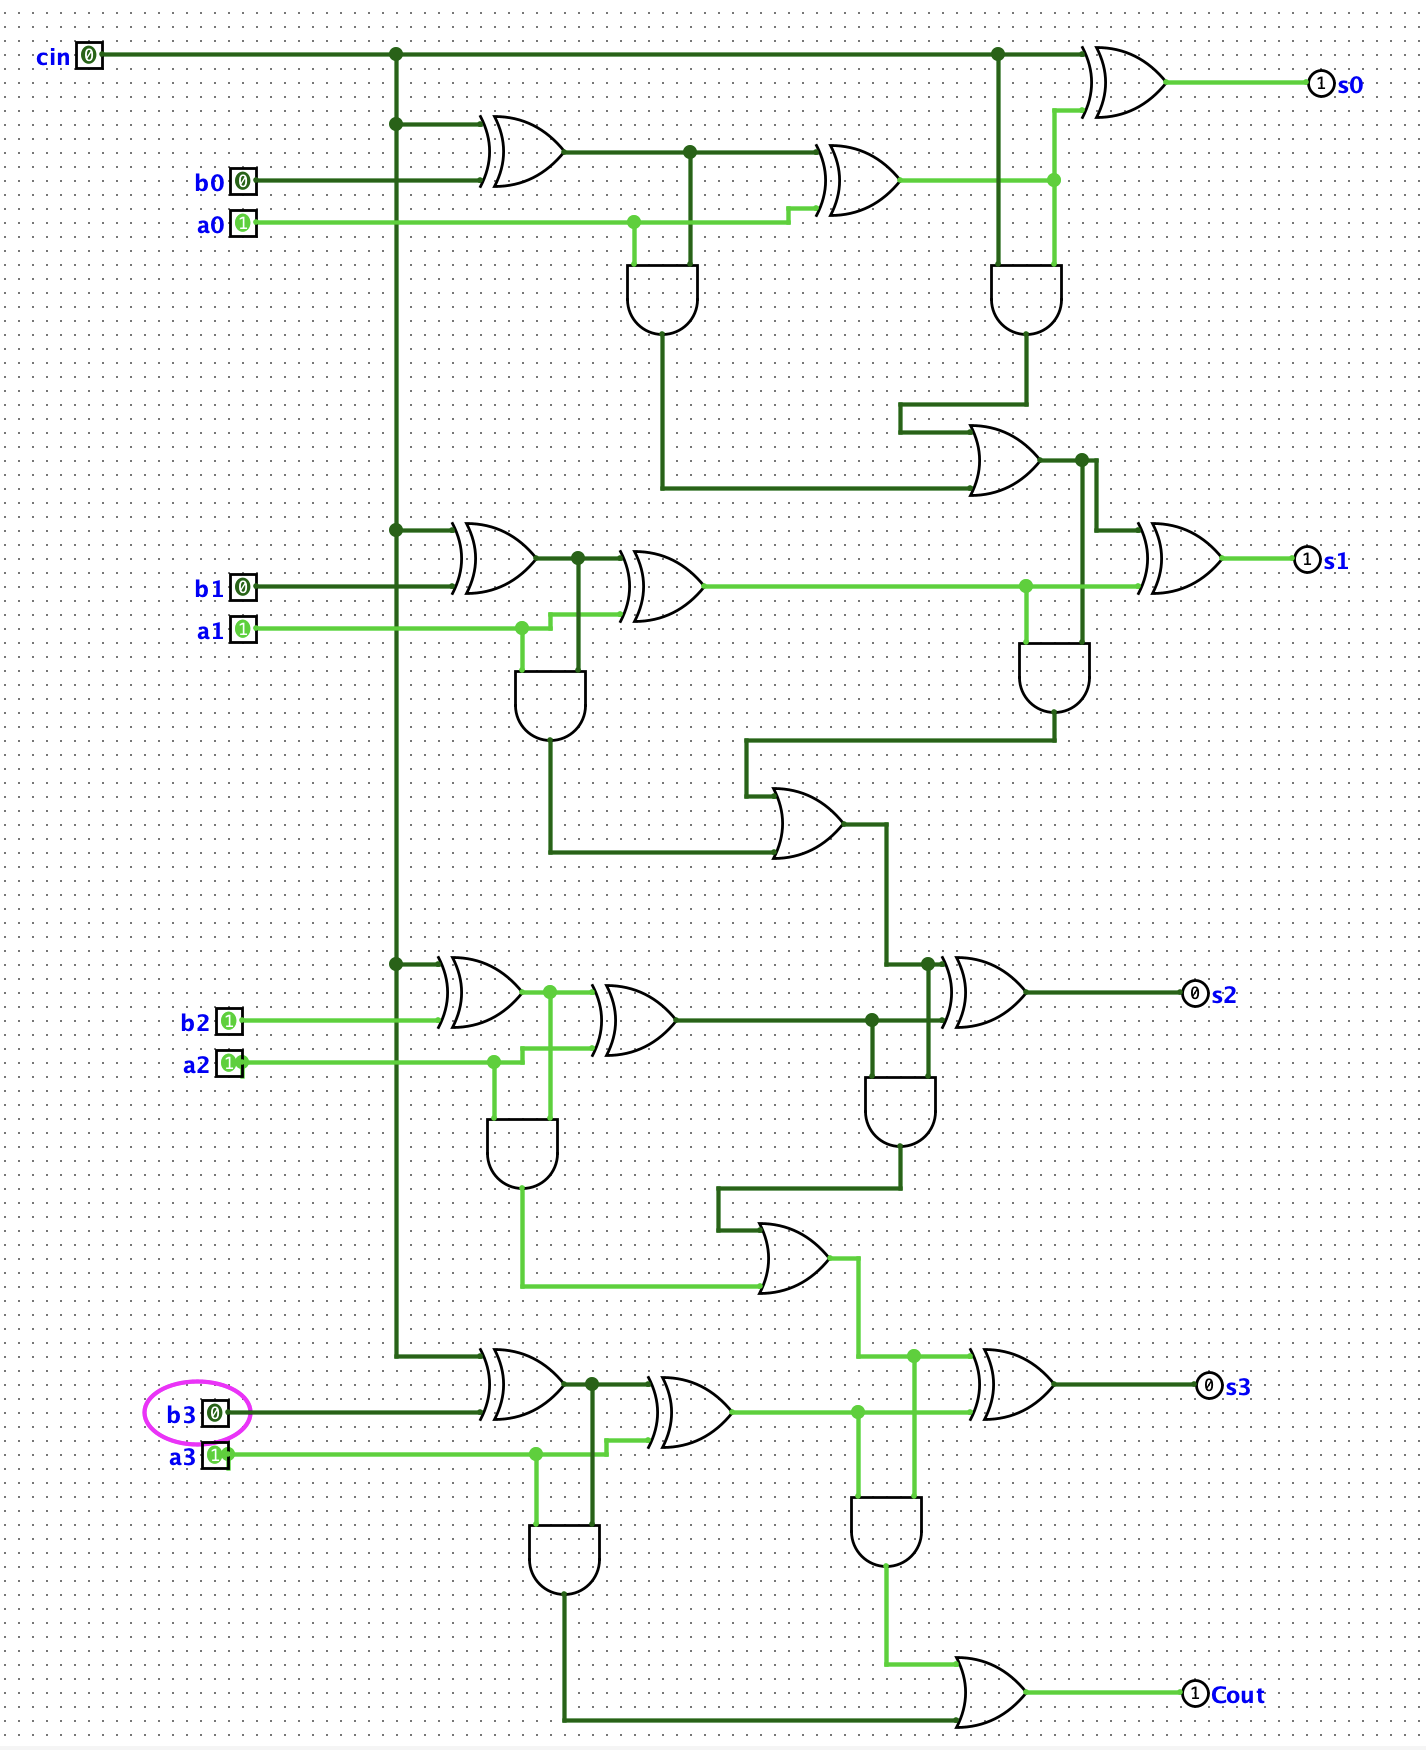
\includegraphics[width=0.9\textwidth]{images/Logisim/ast1.png}
    \caption{}       
    \label{fig:ast1}
\end{figure}

\begin{figure}[htbp]                    
    \centering
    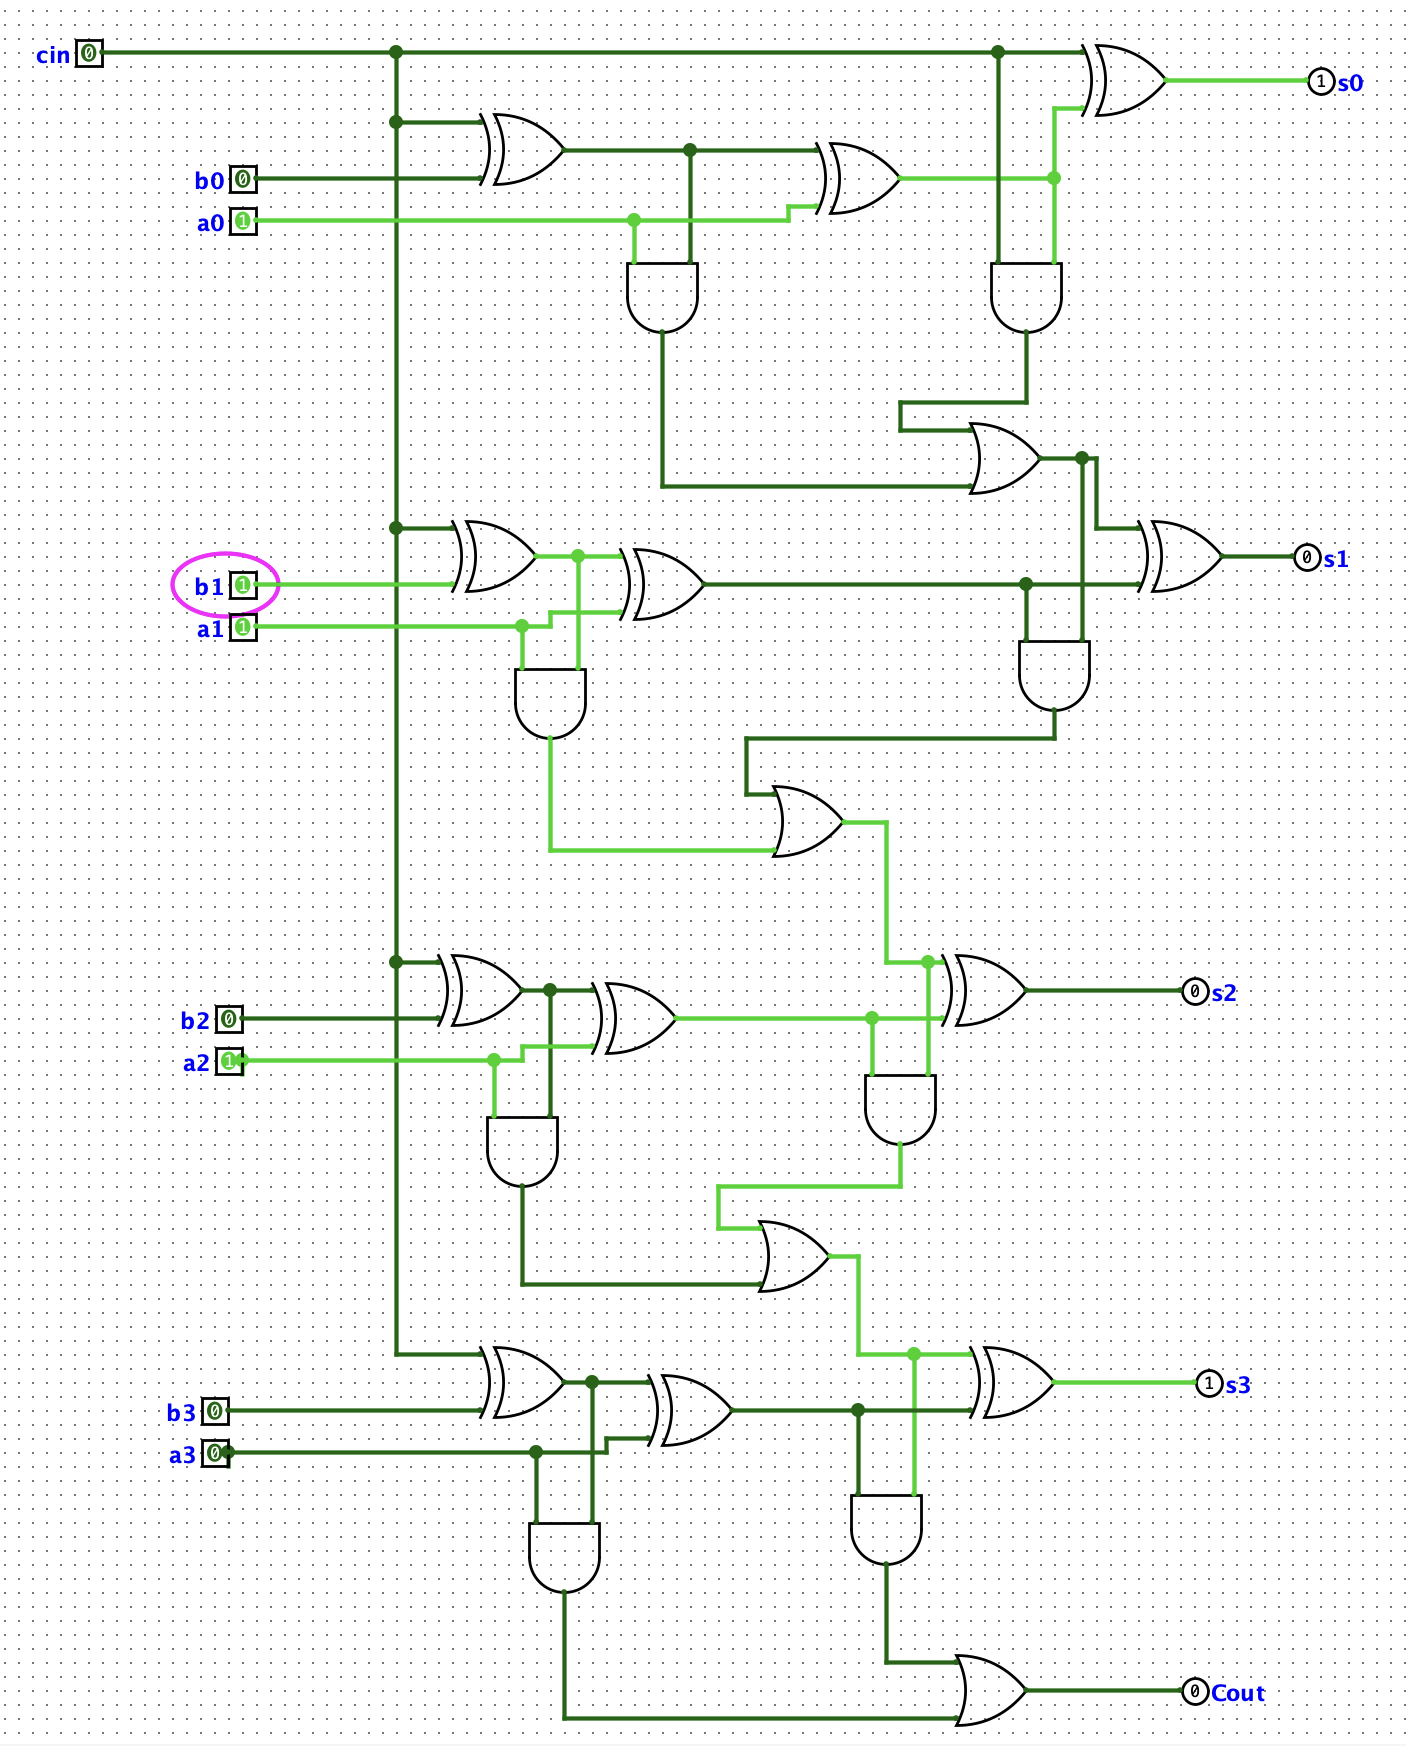
\includegraphics[width=0.9\textwidth]{images/Logisim/ast2.png}
    \caption{}       
    \label{fig:ast2}
\end{figure}

\begin{figure}[htbp]                    
    \centering
    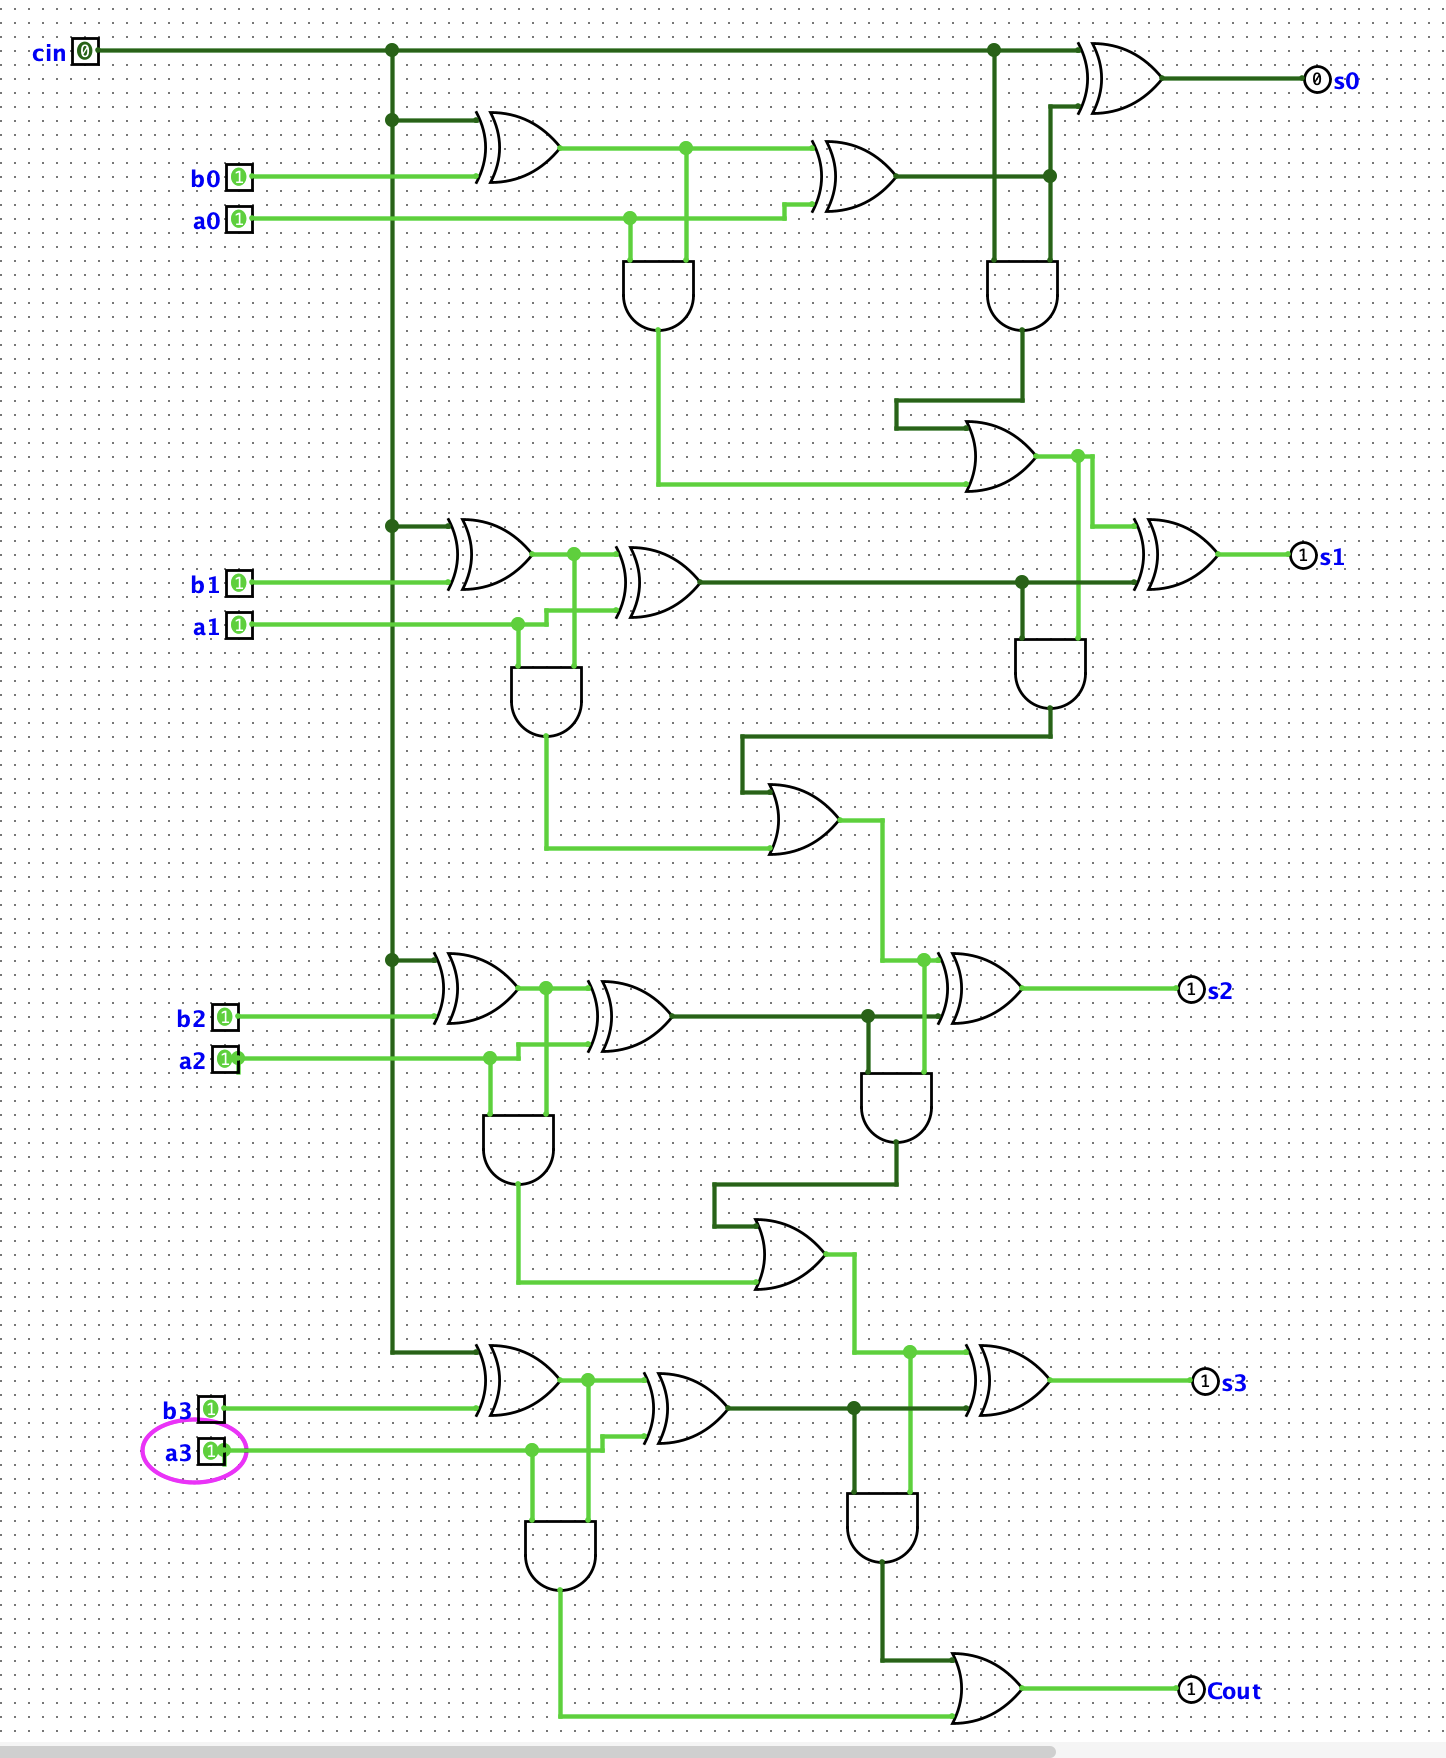
\includegraphics[width=0.9\textwidth]{images/Logisim/ast3.png}
    \caption{}       
    \label{fig:ast3}
\end{figure}

\begin{figure}[htbp]                    
    \centering
    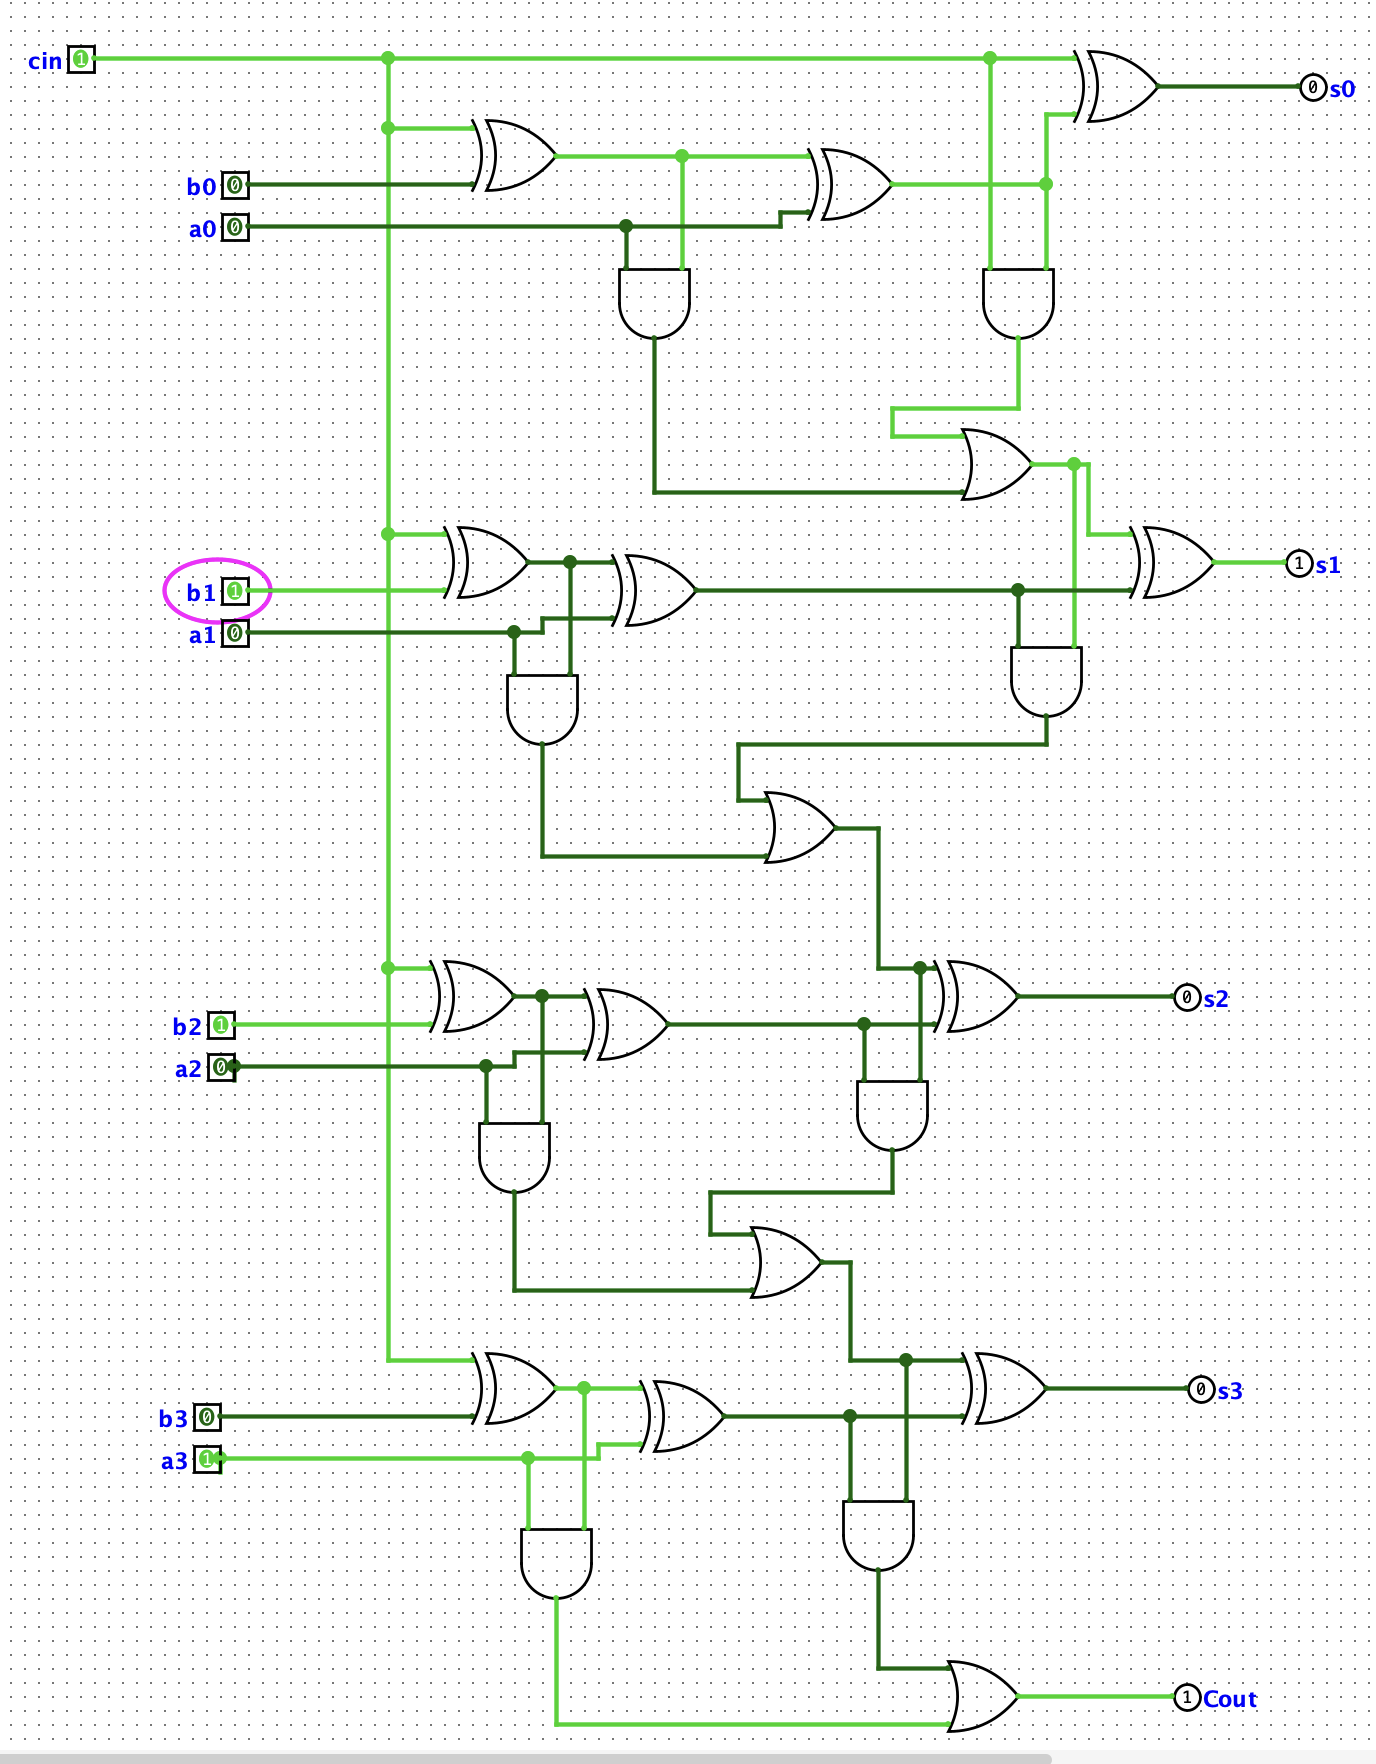
\includegraphics[width=0.9\textwidth]{images/Logisim/ast4.png}
    \caption{}       
    \label{fig:ast4}
\end{figure}

\begin{figure}[htbp]                    
    \centering
    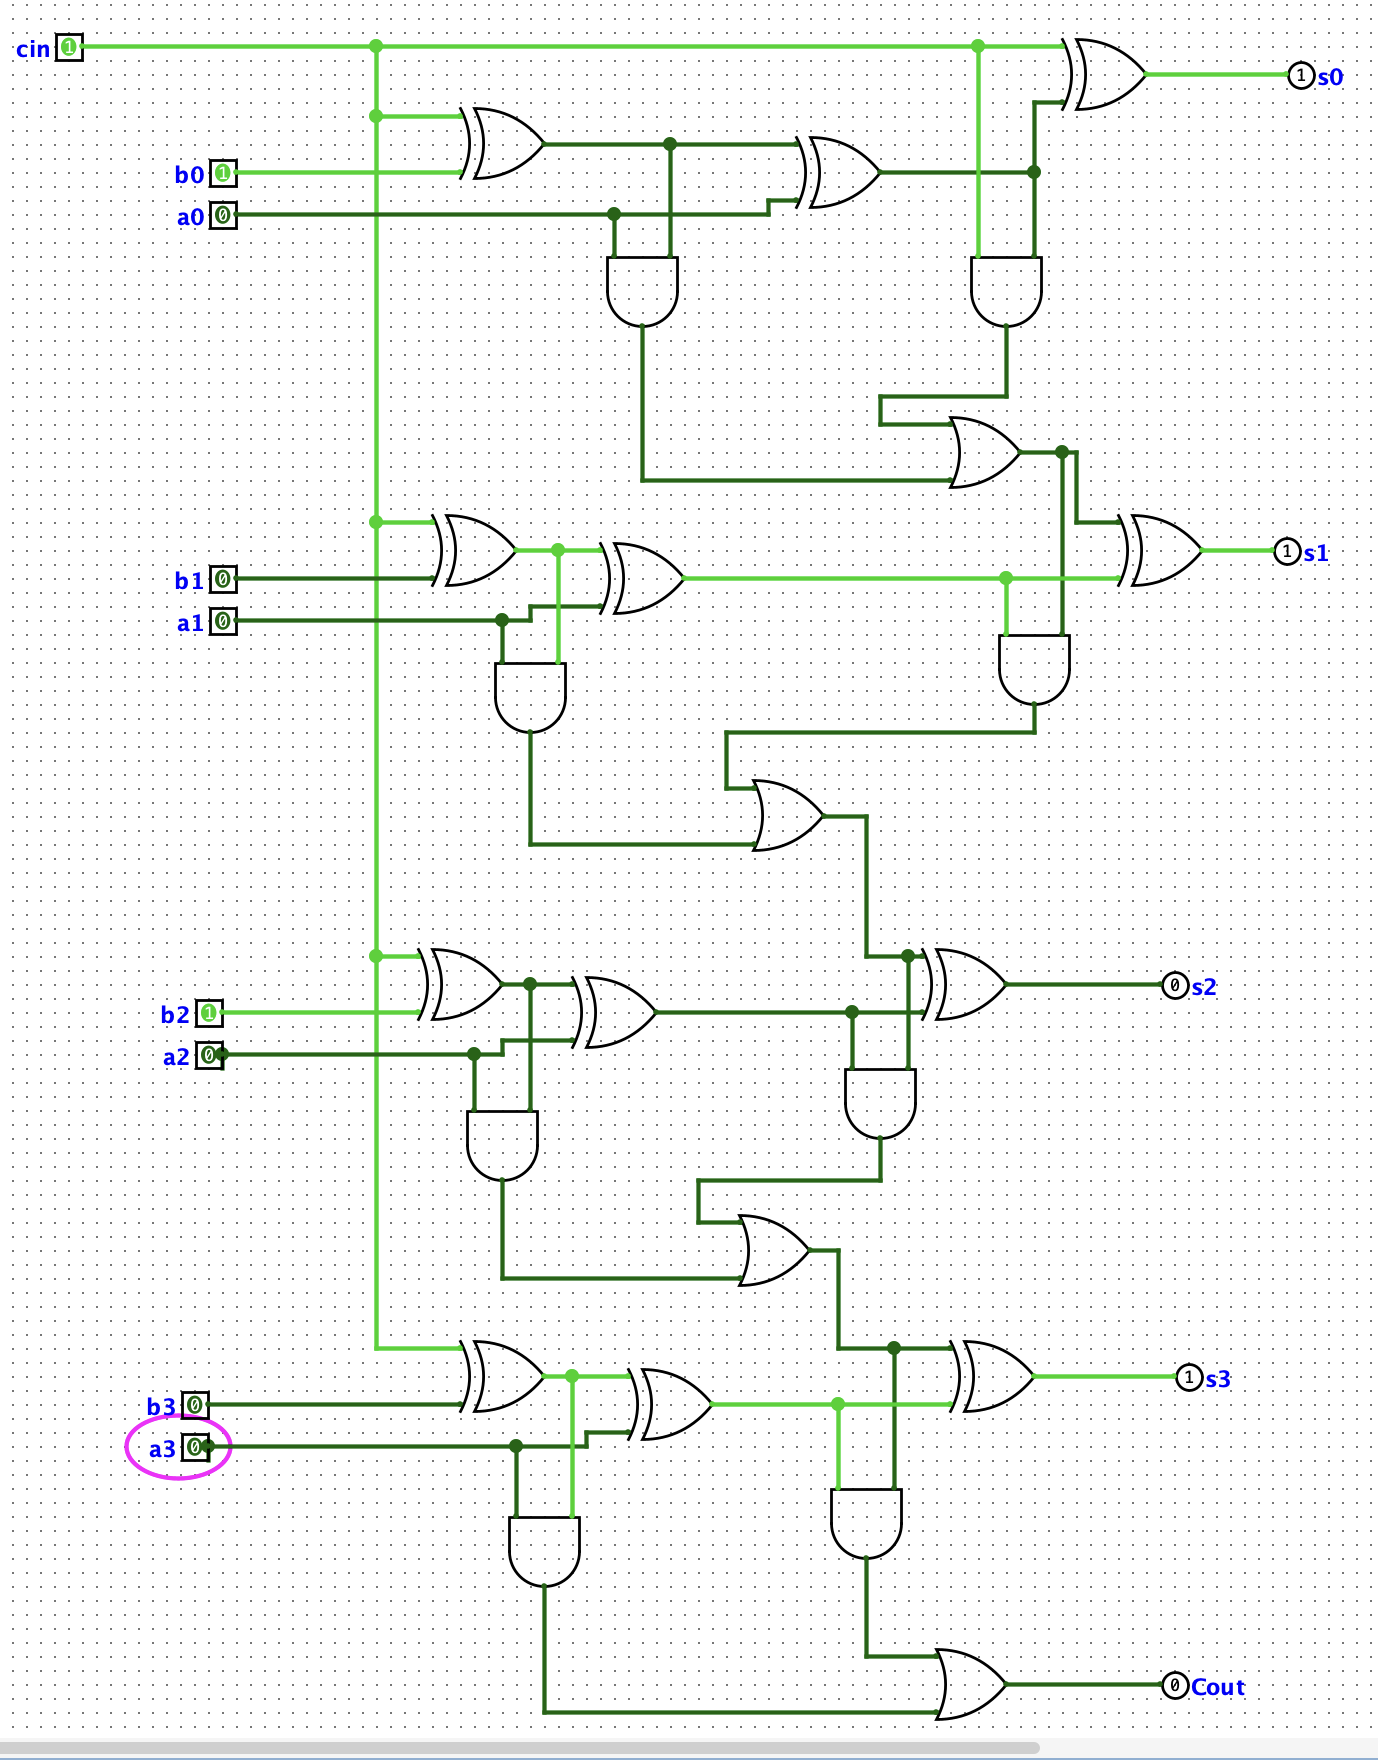
\includegraphics[width=0.9\textwidth]{images/Logisim/ast5.png}
    \caption{}       
    \label{fig:ast5}
\end{figure}

\begin{figure}[htbp]                    
    \centering
    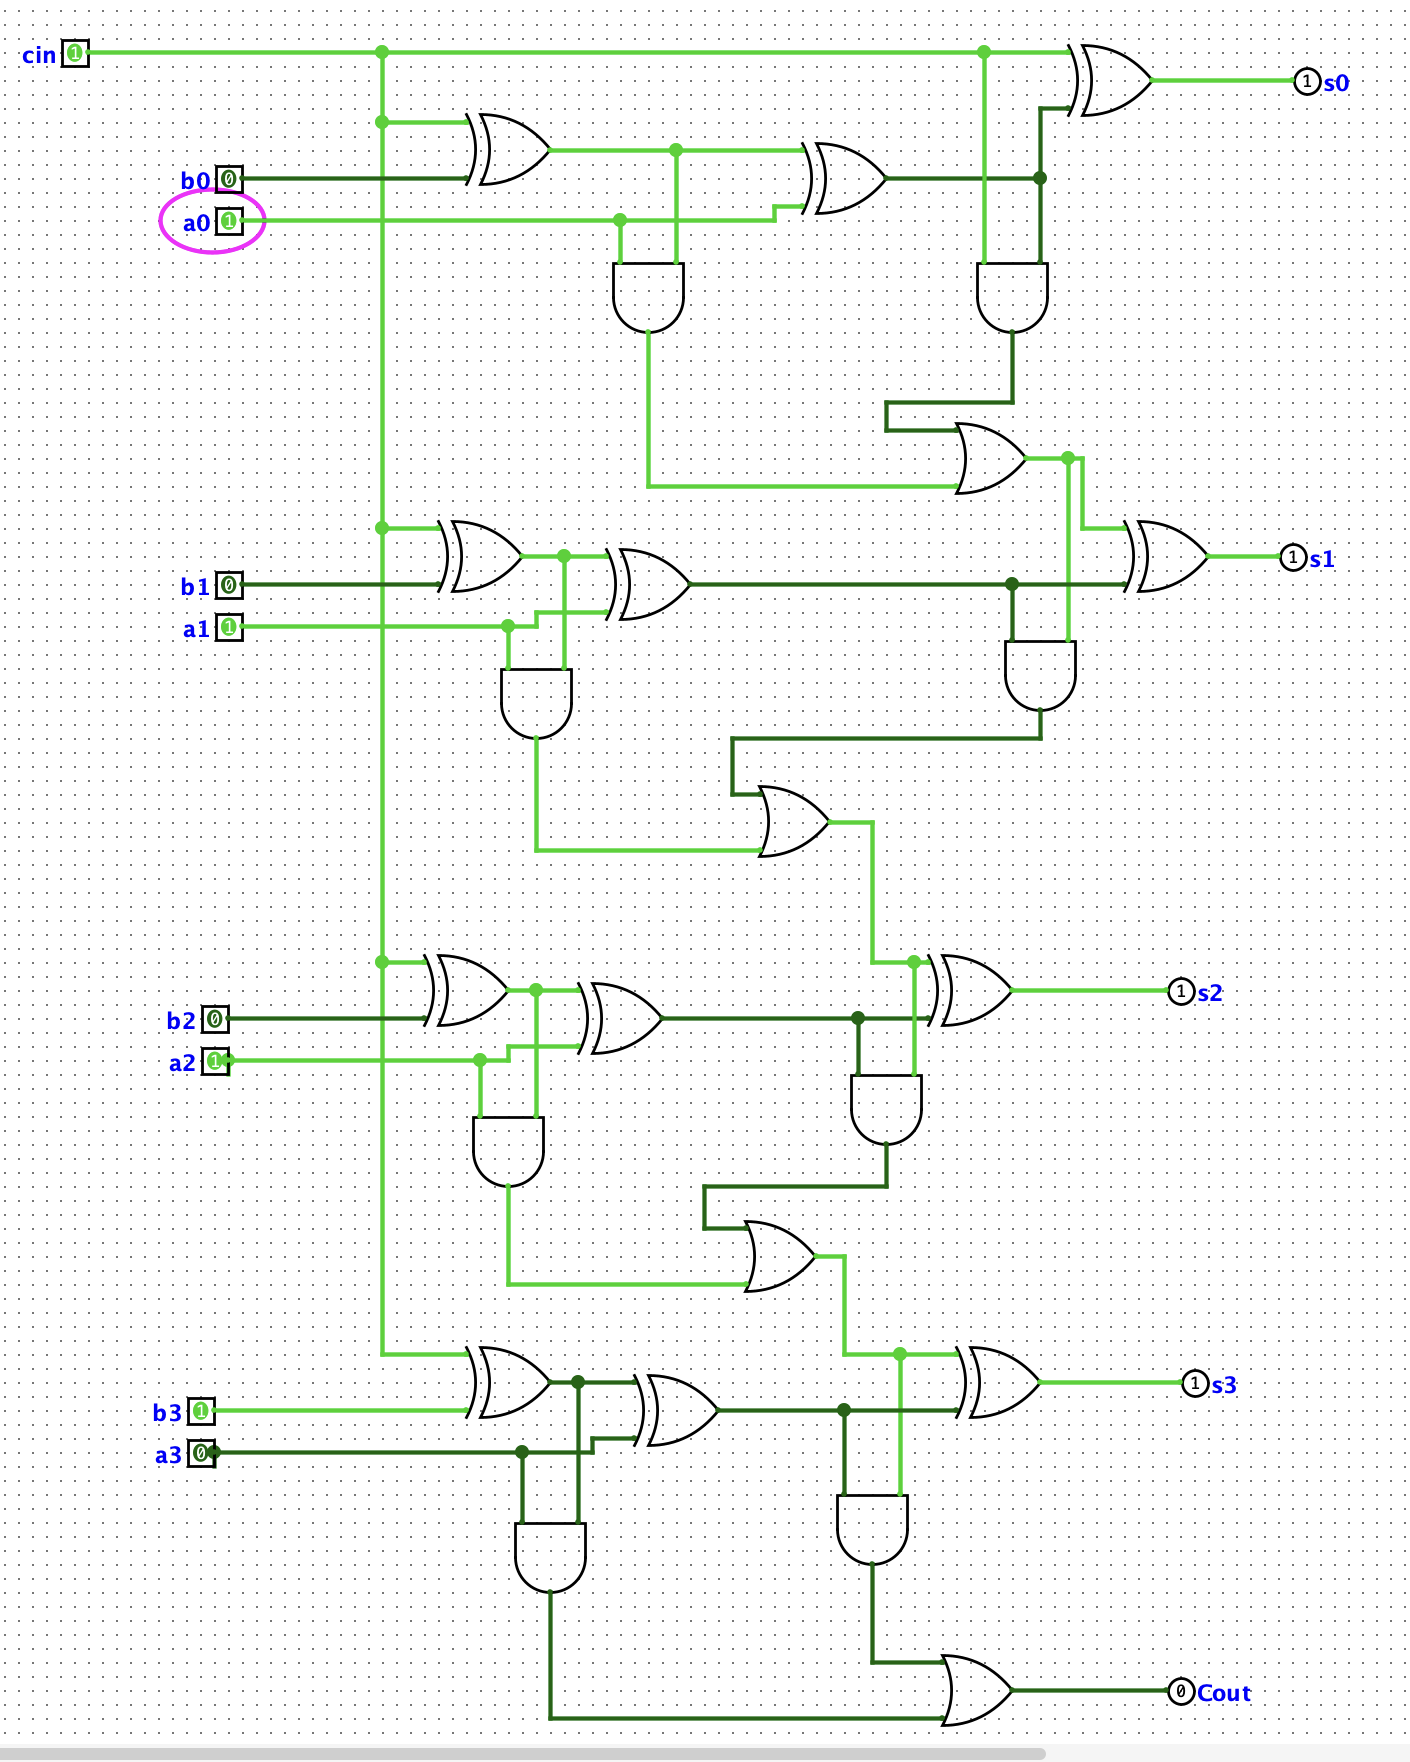
\includegraphics[width=0.9\textwidth]{images/Logisim/ast6.png}
    \caption{}       
    \label{fig:ast6}
\end{figure}

\begin{figure}[htbp]                    
    \centering
    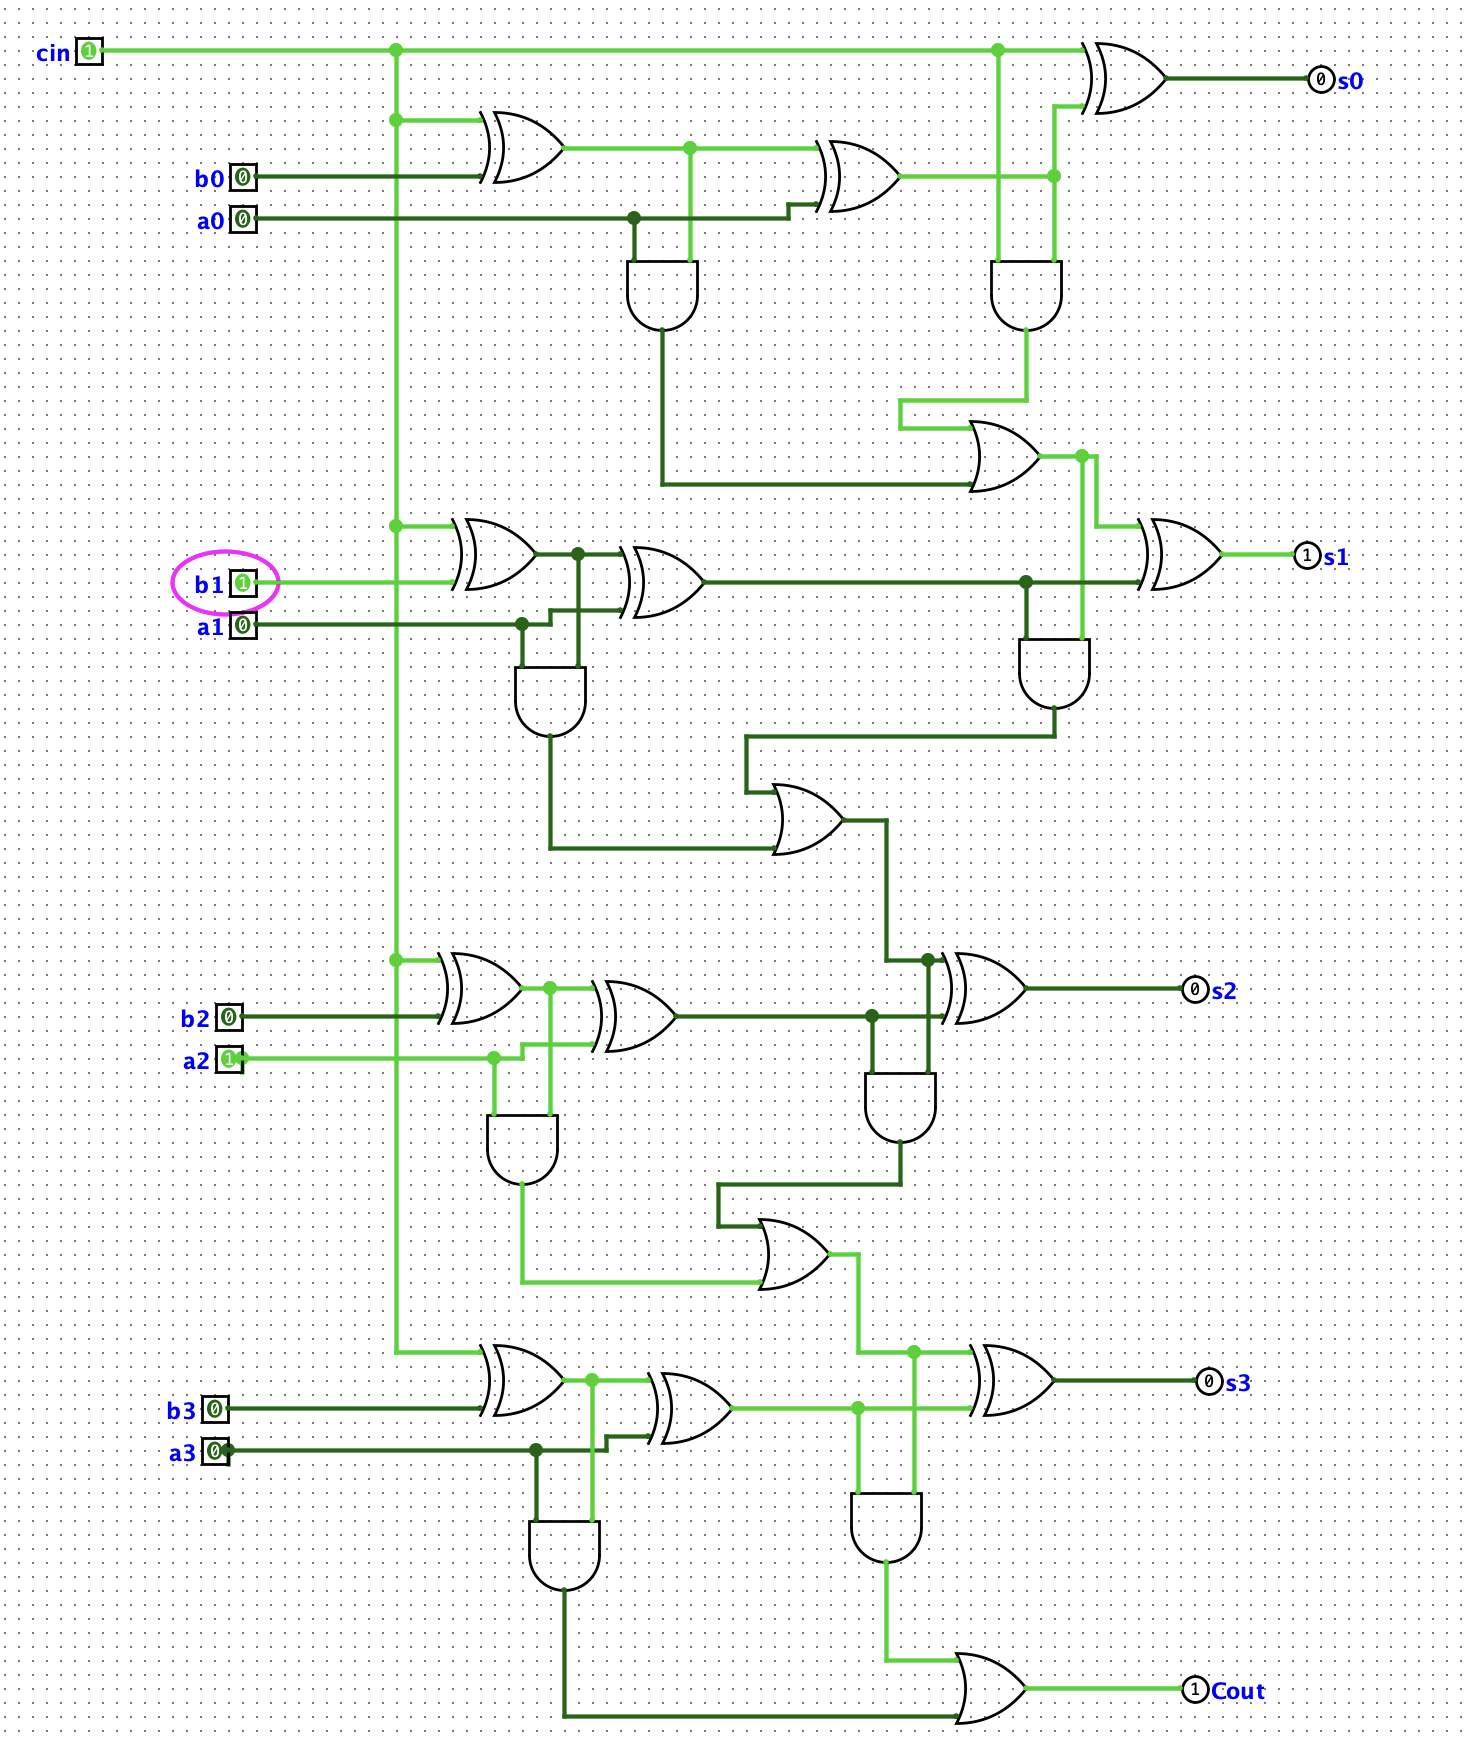
\includegraphics[width=0.9\textwidth]{images/Logisim/ast7.png}
    \caption{}       
    \label{fig:ast7}
\end{figure}

\clearpage

\section{ساخت مدار با \lr{Proteus}}
\leavevmode\par
\vspace{0.3cm}

\begin{spacing}{1.3}
در این قسمت قصد داریم با استفاده از نرم‌افزار \lr{Proteus} یک مدار جمع کننده چهاربیتی از نوع\\ \lr{Carry-Look-Ahead(CLA)} بسازیم.
\end{spacing}

\subsection{طراحی مدار}
\leavevmode\par
\vspace{0.3cm}

\begin{spacing}{1.3}
مدار جمع‌کننده \lr{Carry-Look-Ahead} یک مدار جمع‌کننده پرسرعت است که بر مشکل تاخیر انتشار\LTRfootnote{Propagation Delay} که در جمع‌کننده های \lr{Ripple Carry Adder} وجود دارد غلبه می‌کند. زیرا در جمع‌کننده های \lr{RCA} هر بیت برای محاسبه حاصل جمع نهایی باید منتظر دریافت \lr{Carry} از بیت قبلی بماند. اما در مدار \lr{CLA} تمام ارقام نقلی بیت ها به صورت همزمان و مستقیما از سیگنال های ورودی با استفاده از توابع منظقی تولید می‌شوند.

توابعی که \lr{CLA} با استفاده از آنها ارقام نقلی را پیش‌بینی می‌کند، توابع \lr{Generate(G)} و \lr{Propagate(P)} هستند که به این صورت تعریف می‌شوند:
\end{spacing}

\begin{latin}
$$P_i = a_i \oplus b_i$$
$$G_i = a_i . b_i$$
\end{latin}

\begin{spacing}{1.3}
که اگر شکل مدار جمع‌کننده کامل را با این توابع مقایسه کنیم، نتیجه می‌گیریم می‌توانیم \lr{$S_i$} , \lr{$C_{i+1}$} را از این طریق بدست آوریم:
\end{spacing}

\begin{latin}
$$S_i = P_i \oplus C_i$$
$$C_{i+1} = G_i + P_i . C_i$$
\end{latin}

\begin{spacing}{1.3}
برای مثال، \lr{$C_1$} و \lr{$C_2$} را با استفاده از رابطه بازگشتی بالا بدست می‌آوریم:
\end{spacing}

\begin{latin}
$$C_1 = G_0 + P_0 . C_0$$
$$C_2 = G_1 + P_1 . C_1 = G_1 + P_1(G_0 + P_0 . C_0) = G_1 + G_0 . P_1 + P_1 . P_0 . C_0$$
\end{latin}

\begin{spacing}{1.3}
همانگونه که مشاهده می‌شود، به ازای تعداد بیت های بیشتر، تعداد گیت‎‌های استفاده شده و تعداد ورودی های آنها و در نتیجه پیچیدگی مدار بیشتر می‌شود. در واقع، بهای افزایش سرعت در \lr{CLA} افزایش پیچیددگی(مساحت) مدار است.
\end{spacing}


\begin{figure}[htbp]                    
    \centering
    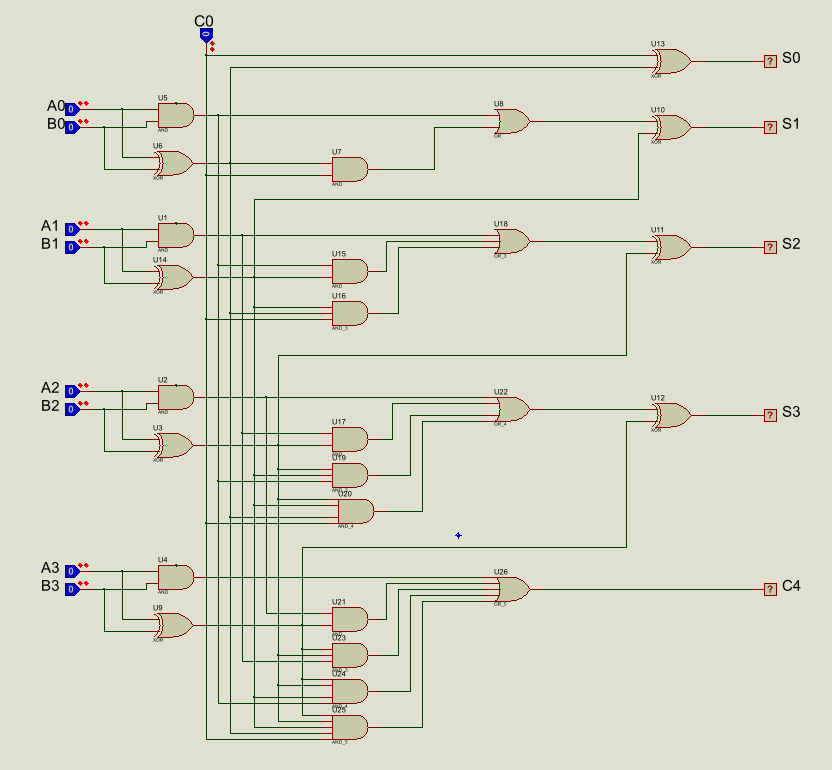
\includegraphics[width=1\textwidth]{images/Proteus/rca.png}
    \caption{مدار جمع‌کننده چهاربیتی \lr{Carry-Look-Ahead}}       
    \label{fig:rca}
\end{figure}

\clearpage

\subsection{تست مدار}
\leavevmode\par
\vspace{0.3cm}

\begin{spacing}{1.3}

شکل \ref{fig:rcat1}:

\begin{latin}
$A = (1101)_2, B = (0010)_2, c_0 = 1$ 

binary: $(1101)_2 + (0010)_2 + 1 = (10000)_2$

decimal: $13 + 2 + 1 = 16$
\end{latin}

شکل \ref{fig:rcat2}:

\begin{latin}
$A = (0001)_2, B = (0001)_2$ 

binary: $(0001)_2 + (0001)_2  = (00010)_2$

decimal: $1 + 1  = 2$
\end{latin}

شکل \ref{fig:rcat3}:

\begin{latin}
$A = (0111)_2, B = (1000)_2$ 

binary: $(0111)_2 + (1000)_2  = (01111)_2$

decimal: $7 + 8  = 15$
\end{latin}

شکل \ref{fig:rcat4}:

\begin{latin}
$A = (1111)_2, B = (1000)_2$ 

binary: $(1111)_2 + (1000)_2 = (10111)_2$

decimal: $15 + 8  = 23$
\end{latin}

\end{spacing}

\begin{figure}[htbp]                    
    \centering
    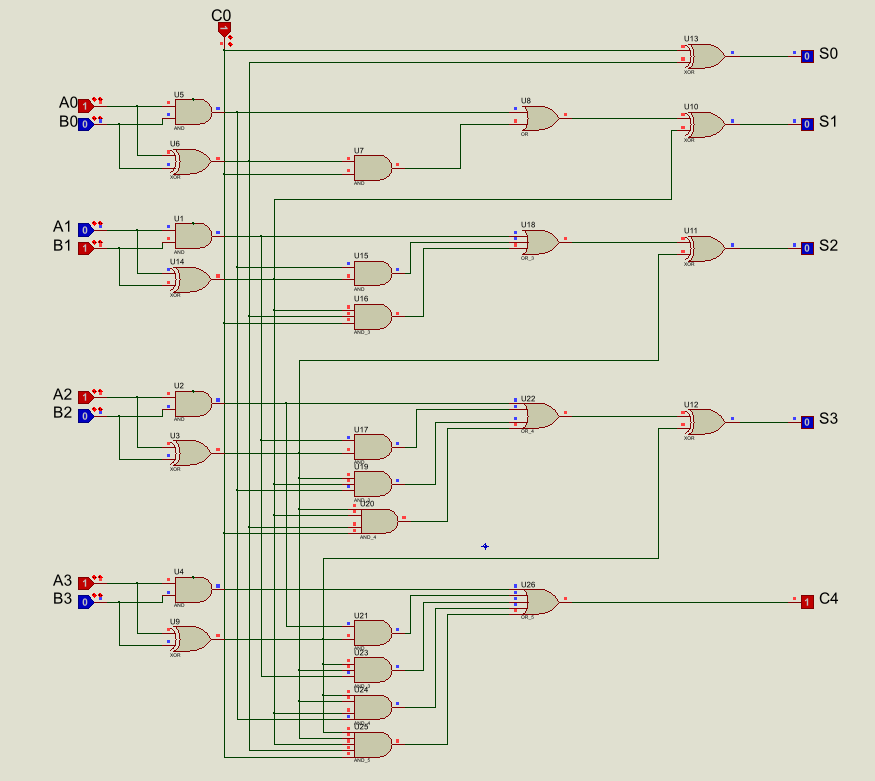
\includegraphics[width=1\textwidth]{images/Proteus/rcat1.png}
    \caption{}       
    \label{fig:rcat1}
\end{figure}

\begin{figure}[htbp]                    
    \centering
    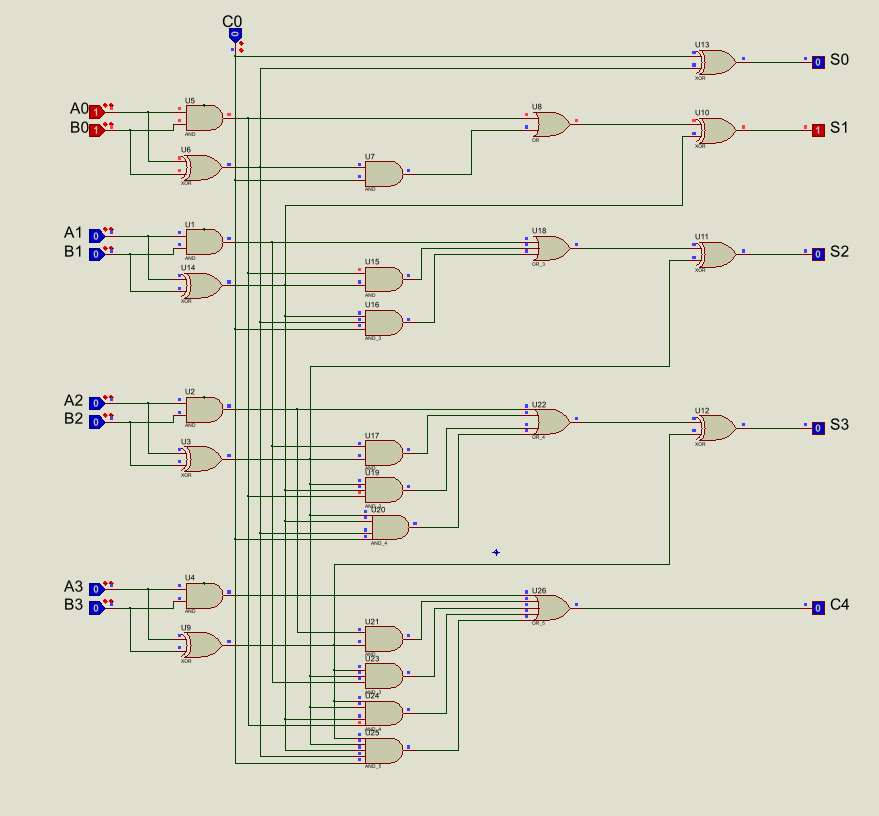
\includegraphics[width=1\textwidth]{images/Proteus/rcat2.png}
    \caption{}       
    \label{fig:rcat2}
\end{figure}

\begin{figure}[htbp]                    
    \centering
    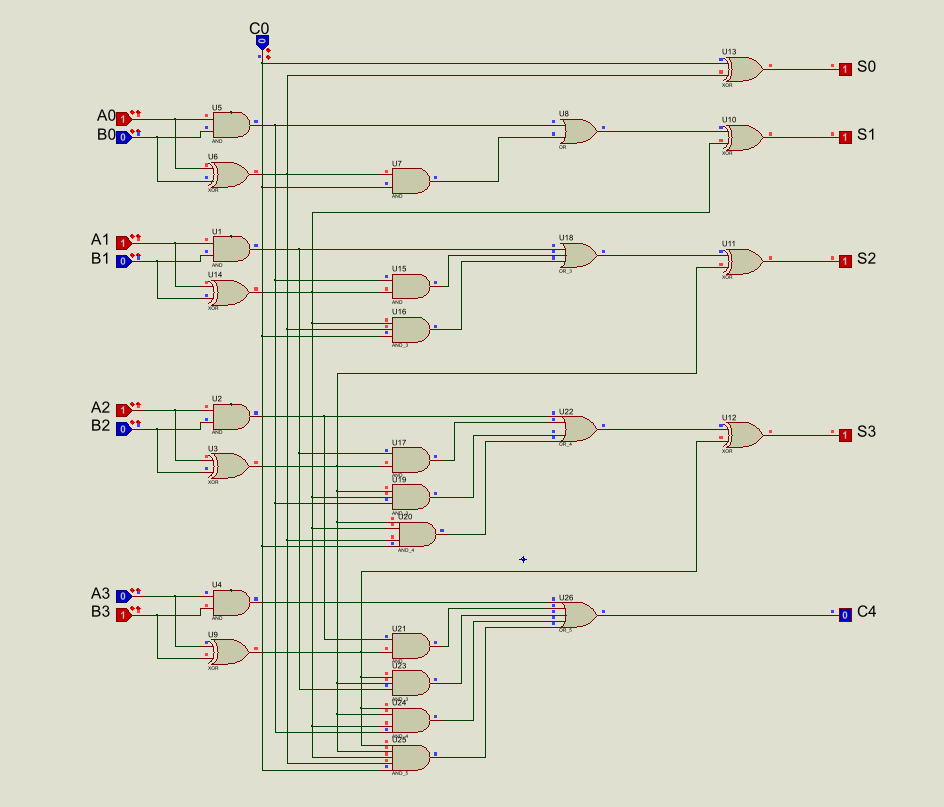
\includegraphics[width=1\textwidth]{images/Proteus/rcat3.png}
    \caption{}       
    \label{fig:rcat3}
\end{figure}

\begin{figure}[htbp]                    
    \centering
    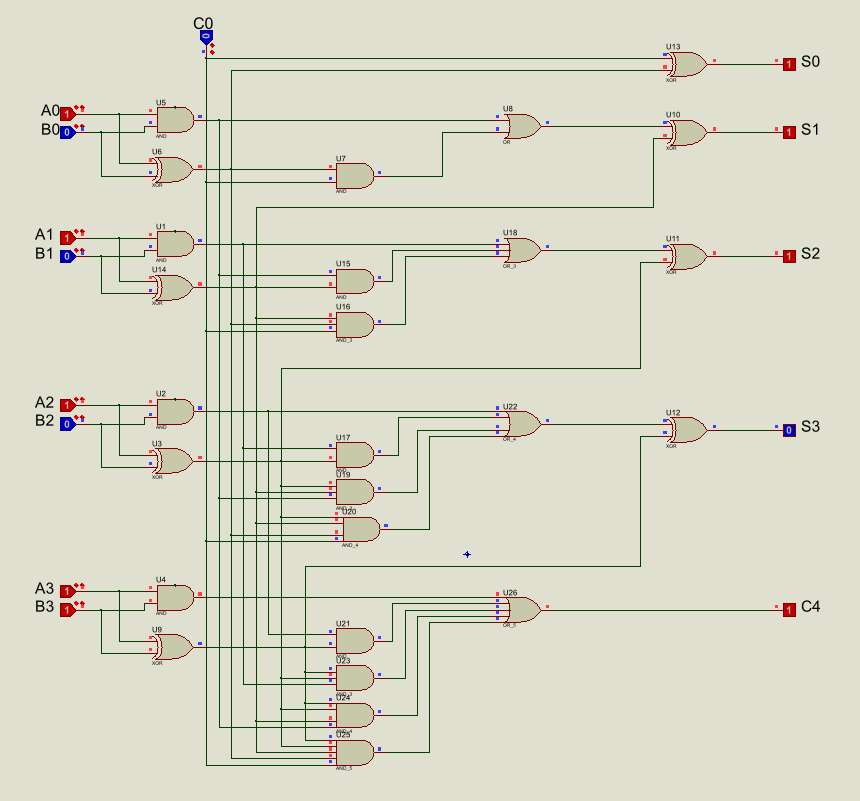
\includegraphics[width=1\textwidth]{images/Proteus/rcat4.png}
    \caption{}       
    \label{fig:rcat4}
\end{figure}

\clearpage

\section{نتیجه‌گیری}
\leavevmode\par
\vspace{0.3cm}


\begin{spacing}{1.3}
در این آزمایش، با محیط‌ها و ابزارهای مختلف شبیه‌سازی مدارهای منطقی از جمله \lr{Fritzing} ،\lr{Logisim}، و \lr{Proteus} آشنا شدیم.
ابتدا با بررسی نحوه عملکرد بردبورد و پیاده‌سازی مدارهای ساده، نحوه قرار دادن قطعات مختلف و تراشه ها را آموختیم و درک درستی از اتصالات فیزیکی و پایه ها بدست آوردیم.
سپس در نر‌م‌افزار \lr{Logisim}، توانستیم مدار جمع‌کننده/تفریق‌کننده جهاربیتی را طراحی و تست کنیم و عمکرد آنرا با محاسبات تئوری تظبیق دهیم.
در نهایت با پیاده‌سازی مدار جمع‌کننده از نوع \lr{Carry-Look-Ahead} با محیط نرم‌افزار به نسبت قدرتمندتر \lr{Proteus} آشنا شدیم.
تمام اهداف این آزمایش به درستی محقق شد و نتایج شبیه‌سازی ها با محاسبات مطابقت داشت.
\end{spacing}


\end{document}